\documentclass[letterpaper, 10 pt, journal, twoside]{IEEEtran}
\IEEEoverridecommandlockouts 
\pdfminorversion=4 
% \documentclass{article}

%\settopmatter{printacmref=false}
\usepackage[colorlinks=true,linkcolor=black,anchorcolor=black,citecolor=black,filecolor=black,menucolor=black,runcolor=black,urlcolor=black]{hyperref}
\usepackage{url}
% \usepackage{icml2021}
%\overrideIEEEmargins 
\usepackage[skip=5pt,font=scriptsize]{caption}
\captionsetup[table]{skip=10pt}
%\usepackage{algorithm2e}% http://ctan.org/pkg/algorithm2e
% \makeatletter
% \newcommand{\nosemic}{\renewcommand{\@endalgocfline}{\relax}}% Drop semi-colon ;
% \newcommand{\dosemic}{\renewcommand{\@endalgocfline}{\algocf@endline}}% Reinstate semi-colon ;
% \newcommand{\pushline}{\Indp}% Indent
% \newcommand{\popline}{\Indm\dosemic}% Undent
% \let\oldnl\nl% Store \nl in \oldnl
% \newcommand{\nonl}{\renewcommand{\nl}{\let\nl\oldnl}}% Remove line number for one line
% \makeatother


\usepackage{graphicx}
%\usepackage{subcaption}
\usepackage{subfigure}
\usepackage{etoolbox}
\usepackage{scalerel}
\usepackage{siunitx}
% \usepackage{pifont}
\usepackage{amsmath,textcomp}
\let\proof\relax
\let\endproof\relax
\usepackage{amssymb}
\usepackage{amsthm}


% 30 dec 2021 shreyas commented these out and uncommented the algorithm2e stuff
% \usepackage{algorithm}
% \usepackage{algorithmicx}
% \usepackage{algpseudocode}
\usepackage[ruled,vlined,linesnumbered]{algorithm2e}
\SetKwInput{KwInput}{Input}
\SetKwInput{KwOutput}{Output}
\SetKwInOut{KwInOut}{Parameter}
\setlength{\algomargin}{0.8em} % required to keep line numbers inside margin

%\usepackage{cite}
% \usepackage{outlines}
% \usepackage{wasysym}
%\usepackage[mathcal]{euscript}
\usepackage{bbm}
%\usepackage{mathptmx}
\usepackage{booktabs}
\usepackage{url}
\usepackage{paralist}
\usepackage{color}
% \usepackage{stmaryrd}
%\usepackage{epsfig}
\usepackage{mathtools}
%\usepackage{mathrsfs}
\usepackage{xspace}
\usepackage{verbatim}
\usepackage{epstopdf}
\usepackage{listings}
\usepackage{lstautogobble}
% \usepackage{parcolumns}
\usepackage[utf8]{inputenc}
\usepackage{calrsfs}
\usepackage{rotating,multirow}


% \usepackage[most]{tcolorbox} % this package prevents clicking in the document to identify the corresponding part of code, see here: https://www.overleaf.com/learn/how-to/SyncTeX_Errors
% \usepackage[T1]{fontenc}
\usepackage[utf8]{inputenc}
\let\labelindent\relax
\usepackage{enumitem}
%\usepackage{authblk}
\usepackage{hyperref}

%\let\nopagenumber\relax
\usepackage{titlesec}
\titlespacing\section{0pt}{3pt}{4pt}
\titlespacing\subsection{0pt}{2pt}{3pt}
\titlespacing\subsubsection{0pt}{1pt}{2pt}

%---- space adjust--------
%%\newcommand{\subparagraph}{}
%%\usepackage[text={16cm,24cm}]{geometry}
%\usepackage{titlesec}
%\titlespacing{\section}{0pt}{0.6ex}{0.5ex}
%\titlespacing{\subsection}{0pt}{0.3ex}{0.3ex}
%\titlespacing{\subsubsection}{0pt}{0.2ex}{0.2ex}

% \setlength{\parskip}{0cm}
% \setlength{\parindent}{1em}
%%\titlespacing*{commandi}{left}{before-sep}{after-sep}[right-sep]
%\usepackage[compact]{titlesec}


% allow divide split equation between two pages
\allowdisplaybreaks

%space after and before equations
\setlength{\abovedisplayskip}{4pt}
\setlength{\belowdisplayskip}{4pt}


% notes
\newcommand{\TODO}[1]{\textcolor{red}{#1}}

% theorem blocks
\newtheorem{definition}{Definition}
\newtheorem{proposition}{Proposition}
\newtheorem{theorem}{Theorem}
\newtheorem{remark}{Remark}
\newtheorem{lemma}{Lemma} 
\newtheorem{assumption}{Assumption} 
\newtheorem{property}{Property}
\newtheorem{corollary}{Corollary}
\renewcommand{\footnotesize}{\fontsize{8pt}{11pt}\selectfont}

% text modifications
\DeclareMathAlphabet{\mathcal}{OMS}{cmsy}{m}{n}
\newcommand{\regtext}[1]{\mathrm{\textnormal{#1}}}
\newcommand{\defemph}[1]{\emph{#1}}
\newcommand{\ts}[1]{\textsuperscript{#1}}

% special characters
\newcommand{\cmark}{\ding{51}}
\newcommand{\xmark}{\ding{55}}
\newcommand{\sm}[1]{\scaleto{#1}{3.5pt}}
\newcommand{\sB}[1]{\scaleto{#1}{5pt}}

% sets
\newcommand{\R}{{\mathbb{R}}}
\newcommand{\Z}{{\mathbb{Z}}}
\newcommand{\B}{{\mathbb{B}}}
\newcommand{\N}{{\mathbb{N}}}
\newcommand{\X}{{\mathbf{X}}}



% operations
%\DeclareMathDelimiter{(}{\mathopen} {operators}{"28}{largesymbols}{"00}
%\DeclareMathDelimiter{)}{\mathclose}{operators}{"29}{largesymbols}{"01}
\DeclarePairedDelimiter\ceil{\lceil}{\rceil}
\DeclarePairedDelimiter\floor{\lfloor}{\rfloor}
\DeclarePairedDelimiter{\abs}{\lvert}{\rvert}
\DeclarePairedDelimiter{\norm}{\lVert}{\rVert}
\DeclareMathOperator*{\argmax}{arg\,max}
\DeclareMathOperator*{\argmin}{arg\,min}
\newcommand{\diag}[1]{\regtext{diag}\!\left(#1\right)}
\newcommand{\comp}{^{\regtext{C}}}
\newcommand{\trans}{^\top}
\newcommand{\opt}{^\star}
\newcommand{\proj}{\regtext{proj}}

% vector thingies
\newcommand{\vc}[1]{{\mathbf{#1}}}

% special matrices and sets
\newcommand{\ones}{\vc{1}}
\newcommand{\emptyarr}{[\ ]}
\newcommand{\zeros}{\vc{0}}
\newcommand{\eye}{\vc{I}}
\newcommand{\zono}[1]{\mathcal{Z}\!\left(#1\right)}
% \newcommand{\zono}[1]{\left\langle#1\right\rangle} % original shorthand
\newcommand{\conzono}[1]{\mathcal{CZ}\!\left(#1\right)}
\newcommand{\matzono}[1]{\mathcal{MZ}\!\left(#1\right)}
\newcommand{\polytope}[1]{\mathcal{P}\!\left(#1\right)}

% zonotope objects
% Mahmoud: replaced \vc with \textbf
\newcommand{\ctr}{\vc{c}}
\newcommand{\Ctr}{\vc{C}}
\newcommand{\gen}{\vc{g}}
\newcommand{\Gen}{\vc{G}}
\newcommand{\Acon}{\vc{A}}
\newcommand{\bcon}{\vc{b}}
\newcommand{\coef}{\vc{z}}
\newcommand{\lb}{\underline{\vc{l}}}
\newcommand{\ub}{\overline{\vc{l}}}

% indices
\newcommand{\idx}[1]{^{(#1)}}
% \newcommand{\arridx}[1]{\!\left[#1\right]}
\newcommand{\arridx}[2]{{\left(#1\right)}_{#2}}
% \newcommand{\arridx}[2]{#1\!\left[#2\right]}
\newcommand{\idxi}{\idx{i}}
\newcommand{\idxj}{\idx{j}}
\newcommand{\idxn}{\idx{n}}
\newcommand{\idxm}{\idx{m}}
\newcommand{\tidx}[1]{_{#1}}

% labels
\newcommand{\lbl}[1]{_{\regtext{#1}}}
\newcommand{\obs}{\lbl{obs}}
\newcommand{\goal}{\lbl{goal}}
\newcommand{\miss}{\lbl{miss}}
\newcommand{\safe}{\lbl{safe}}
\newcommand{\pnlty}{\lbl{pen}}
\newcommand{\total}{\lbl{total}}
\newcommand{\brk}{\lbl{brk}}
\def \tr{\textcolor{red}}
\def \tb{\textcolor{black}}
\newcommand{\tbold}[1]{#1}

% numbers of things
\newcommand{\ngen}{{n\lbl{g}}}
\newcommand{\ncon}{{n\lbl{c}}}
\newcommand{\nrl}{{n\lbl{RL}}}
\newcommand{\nepisodes}{{n\lbl{ep}}}
\newcommand{\niter}{{n\lbl{iter}}}
\newcommand{\ndream}{{n\lbl{dream}}}
\newcommand{\nplan}{{n\lbl{plan}}}
\newcommand{\nbrk}{{n\brk}}
\newcommand{\ntraj}{{q}}
\newcommand{\nnoisegen}{{n_{\regtext{g},\noise}}}

% special vectors, functions, and sets
\newcommand{\dyn}{\vc{f}}
\newcommand{\vcstate}{\vc{x}}
\newcommand{\action}{\vc{u}}
\newcommand{\plan}{\vc{p}}
\newcommand{\noise}{\vc{w}}
\newcommand{\statespace}{X}
\newcommand{\actionspace}{U}
\newcommand{\noisespace}{W}
\newcommand{\statedata}{\vc{X}}
% \newcommand{\actiondata}{\vc{U}_{-}}
\newcommand{\actiondata}{\vc{U}_-}
\newcommand{\noisedata}{\vc{W}_{-}}
% \newcommand{\data}{D}
\newcommand{\data}{(\statedata_-,\statedata_+,\actiondata)}
\newcommand{\RLstate}{\hat{\vcstate}}
% \newcommand{\RLaction}{\hat{\action}}
\newcommand{\RLaction}{\action}
\newcommand{\policy}{\pi}
\newcommand{\mimic}{\mu}
\newcommand{\dreamstate}{\tilde{\vcstate}}
\newcommand{\mimicaction}{\tilde{\action}}
\newcommand{\rewfunc}{\rho}
\newcommand{\rew}{r}
\newcommand{\totaltime}{{n\lbl{total}}}
\newcommand{\dreamfunc}[1]{\regtext{dream}\!\left(#1\right)}
\newcommand{\adjustfunc}[1]{\regtext{adjust}\!\left(#1\right)}

% reachability
\newcommand{\reachset}{R}
\newcommand{\reachapprox}{{\hat{\reachset}}}
\newcommand{\reachfunc}[1]{\regtext{reach}\!\left(#1\right)}


\begin{document}

% \twocolumn[
% \icmltitle{
%     Safe Reinforcement Learning for Mobile Robot Navigation using Black-Box Reachability Analysis}
    
\title{Safe Reinforcement Learning Using Black-Box Reachability Analysis}

\author{Mahmoud Selim$^{1}$, Amr Alanwar$^{2}$, Shreyas Kousik$^{3}$, Grace Gao$^{3}$,
Marco Pavone$^{3}$, and Karl H. Johansson$^{4}$
\thanks{Manuscript received: Feb 24, 2022; Revised:
May 11, 2022; Accepted: June 12, 2022}
\thanks{This paper was recommended for publication by
Editor Jens Kober upon evaluation of the Associate Editor and Reviewers’
comments}
\thanks{This work was supported by the Swedish Research Council, and the Knut and Alice Wallenberg Foundation.
Toyota Research Institute provided funds to support this work.
The NASA University Leadership initiative (grant \#80NSSC20M0163) provided funds to assist the authors with their research, but this article solely reflects the opinions and conclusions of its authors and not any NASA entity.}
\thanks{$^{1}$Ain Shams University, Cairo, Egypt.
$^{2}$Jacobs University, Bremen, Germany.
$^{3}$Stanford University, Stanford, CA, USA.
$^{4}$KTH Royal Institute of Technology, Stockholm, Sweden.
Corresponding author: \texttt{mahmoud.selim@eng.asu.edu.eg}.}
\thanks{Digital Object Identifier (DOI): see top of this page}

}

\markboth{IEEE Robotics and Automation Letters. Preprint Version. Accepted June, 2022}
{Selim \MakeLowercase{\textit{et al.}}: BLACK-BOX REACHABILITY-BASED SAFETY} 

\maketitle
%\pagestyle{plain} % SET TO "EMPTY" TO REMOVE PAGE NUMBERS

\begin{abstract}
Reinforcement learning (RL) is capable of sophisticated motion planning and control for robots in uncertain environments.
However, state-of-the-art deep RL approaches typically lack safety guarantees, especially when the robot and environment models are unknown.
To justify widespread deployment, robots must respect safety constraints without sacrificing performance. 
Thus, we propose a Black-box Reachability-based Safety Layer (BRSL) with three main components: (1)~data-driven reachability analysis for a black-box robot model, (2)~a trajectory rollout planner that predicts future actions and observations using an ensemble of neural networks trained online, and (3)~a differentiable polytope collision check between the reachable set and obstacles that enables correcting unsafe actions.
In simulation, BRSL outperforms other state-of-the-art safe RL methods on a Turtlebot 3, a quadrotor, a trajectory-tracking point mass, and a hexarotor in wind with an unsafe set adjacent to the area of highest reward.
\end{abstract}
\begin{IEEEkeywords}
Reinforcement Learning, Robot Safety, Task and Motion Planning
\end{IEEEkeywords}
%\vspace{}
\section{Introduction}
In reinforcement learning (RL), an agent perceives and reacts to consecutive states of its environment to maximize long-term cumulative expected reward \cite{book:sutton1998introduction}. %in a receding-horizon framework.
One key challenge to the widespread deployment of RL in safety-critical systems is ensuring that an RL agent's policies are safe, especially when the system environment or dynamics are a black box and subject to noise \cite{mihatsch2002risk,garcia2015comprehensive}. %garcia2020teaching, koppejan2011neuroevolutionary,
In this work, we consider RL for guaranteed-safe navigation of mobile robots, such as autonomous cars or delivery drones, where safety means collision avoidance.
We leverage RL to plan complex action sequences in concert with data-driven reachability analysis to guarantee safety for a black-box system.

\begin{figure}[t]
    \centering
    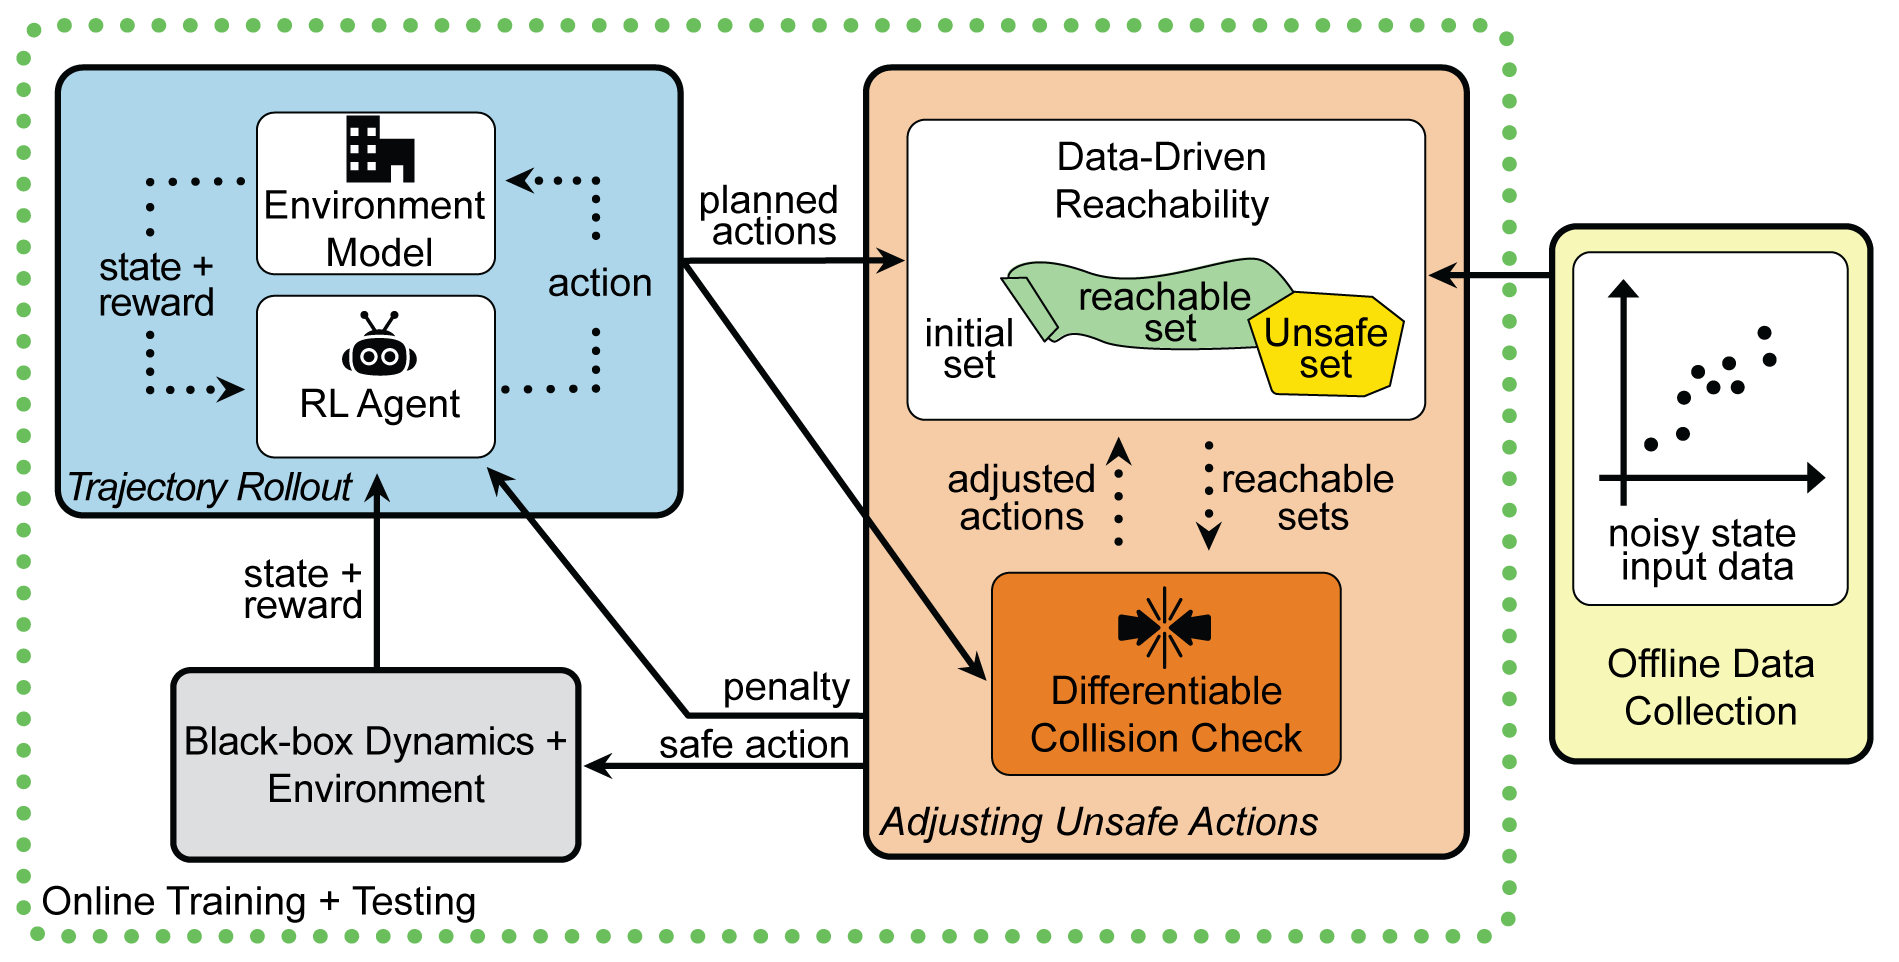
\includegraphics[width=\columnwidth]{Figures/20210922_BRSL-04.png}
    \vspace{-5mm}
    \caption{Overview of the proposed BRSL method (\href{https://youtube.com/playlist?list=PL7bkcpwNaUjz-S1b5KBzpgCZ1SP4DXsoi}{\textcolor{blue}{link to video}}).
    Given data collected offline (in yellow, right), we perform online safe training and deployment of an RL agent.
    The RL agent creates trajectory plans for a robot in a receding-horizon way as follows.
    Each planning iteration is one clockwise loop in the green dashed box.
    First (blue, top left), the agent predicts a possible future trajectory by rolling out its current policy with an ensemble of neural networks trained online to model the black-box environment (grey, bottom left).
    Second (orange, middle), the candidate plan is \emph{adjusted} to ensure safety using data-driven reachability and a constrained, differentiable method of collision-checking our robot's reachable sets.
    We execute a failsafe maneuver if the collision check is infeasible.
    Finally, the new safe plan is passed to the robot, and a penalty is passed to the RL agent for choosing unsafe action.}
    \label{fig:framework}
    \vspace{-6mm}
\end{figure}










\subsection{Related Work} \label{sec:related}
%\textbf{Related Work.}
%Safety has long been of interest in RL research. %Unlike traditional RL, 
Safe RL aims to learn policies that maximize expected reward on a task while respecting safety constraints during both learning and deployment \cite{garcia2015comprehensive}. 
Existing methods can be roughly classified as \emph{objective-based} or \emph{exploration-based}, depending on how safety is formulated.
We first discuss these categories, then the specific case of mobile robot navigation, which we use to evaluate our proposed method.

Objective-based methods encourage safety by penalizing constraint violations in the objective.
This can be done by relating cumulative reward to the system's risk, such as the probability of visiting error states \cite{geibel2005risk}.
In practice, this results in an RL agent attempting to minimize an empirical risk measure (that is, an approximation of the probability of entering a dangerous or undesired state).
Similarly, one can penalize the probability of losing reward (by visiting an unsafe state) for a given action \cite{mihatsch2002risk}, in which case the agent minimizes temporal differences in the reward and thus also minimizes risk.
Another approach is to restrict policies to be ergodic with high probability, meaning any state can eventually be reached from any other state \cite{moldovan2012safe}.
This is a more general problem, which comes at a cost: feasible safe policies do not always exist, and the algorithms are far more complex. 
While these methods can make an agent prefer safe actions, they cannot guarantee safety during training or deployment.
Another group of objective-based algorithms aims to modify the Markov Decision Process (MDP) that the RL agent tries to optimize.
Some model safe optimization problems as maximizing an unknown expected reward function \cite{pmlr-v37-sui15}.
However, they exploit regularity assumptions on the function wherein similar decisions are associated with similar rewards.
They also assume the bandit setting, where decisions do not cause state transitions.
% Others utilize constrained MDPs to enforce safety \cite{altman1999constrained}.
% These can be broadly classified as either offline or online approaches.
% Offline approaches \cite{achiam2017constrained,bharadhwaj2021conservative} collect data first, then perform the optimization.
% These methods can be quite conservative and hard to scale.
% Online methods \cite{BORKAR2005207,chow2017riskconstrained,bohez2019value}, on the other hand, couple both the data collection and optimization.
% However, they do not guarantee safety in training.
Others utilize constrained MDPs \cite{altman1999constrained} to enforce safety in various RL settings, either online or offline.
Online methods learn by coupling the iteration of numerical optimization algorithms (such as primal-dual gradient updates) with data collection \cite{BORKAR2005207,chow2017riskconstrained,tessler2018reward,bohez2019value}.
These algorithms have also been studied in exploration-based settings \cite{ding2020provably,efroni2020explorationexploitation}.
However, they provide no guarantees on safety during training.
On the other hand, offline schemes separate optimization and data collection \cite{achiam2017constrained,bharadhwaj2021conservative}.
They conservatively enforce safety constraints on every policy iteration but are more challenging to scale up.


Exploration-based methods modify the agent's exploration process instead of its optimization criterion.
Exploration is the process of learning about unexplored states by trying random actions or actions that are not expected to yield maximum reward (for example, an $\epsilon$-greedy strategy).
However, visiting unexplored states na\"ively can harm a robot or its environment.
To avoid this, one can aim to guarantee safety during both exploration and exploitation, in both training and testing, by modifying the exploration strategy to incorporate risk metrics \cite{riskmetricsRL}.
One can also use prior knowledge as an inductive bias for the exploration process \cite{garcia2015comprehensive,neuroevolutionaryinproceedings}; for example, one can provide a finite set of demonstrations as guidance on the task \cite{abbeel2005exploration}.
\tb{
Other approaches use control theory to guide or constrain the RL agent's actions.
Most of these approaches use system models with Lyapunov or control barrier functions (CBFs) to guarantee safety (or stability) of the system \cite{molnar2021model, liu2022robot, chow2018lyapunov}.
One can also combine data-driven approaches with model-free barrier or intervention functions \cite{cheng2019end, modelfreecbfsIVM, wagener2021safe}, or use robust CBFs to model uncertain parts of a system \cite{robustCBFarticle, cbfforunmodeleddynamics}.
Although these approaches can provide strong guarantees, most assume the system is control-affine, and need prior knowledge on some or all of the system model \cite{saferlforchanginglanes,conf:modelBasedReachRL,LewEtAl2021}, which may not always be feasible.
Finally, our method is most similar to \cite{dalal2018safe}, which learns a safety signal from data offline, then uses it to adjust an RL agent's controls at runtime.
This method uses a first-order safety approximation for fast adjustment, but (as we show) can be conservative.
}
 
%\subsection{Robot Navigation using Safe RL }
\tb{
Safe navigation is a fundamental challenge in robotics, because robots typically have uncertain, nonlinear dynamics.
Classical techniques such as A$^*$ or RRT \cite[Ch. 5]{lavalle2006planning} have been proposed to solve the navigation problem without learning.
With these methods, safety has been enforced at different levels of the planning hierarchy, such as trajectory planning \cite{kousik2020bridging}, or low-level control \cite{leung2020infusing}.
More recently, however, learning-based methods have been proposed \cite{saferlforchanginglanes,conf:modelBasedReachRL,LewEtAl2021}.
Some safe RL navigation approaches depend on learning a value function of the expected time that an agent takes to reach the desired goal \cite{chen2016decentralized, chen2018socially}.
Other approaches depend on learning the actions of the robot in an end-to-end manner \cite{long2018optimally, e2efirst, tai2018socially}, meaning that the agent attempts to convert raw sensor inputs (e.g., camera or LIDAR) into actuator commands.
The key advantage of RL over traditional planners is in accelerating computation time and solution quality. %by learning from past experience.
}



\subsection{Proposed Method and Contributions}
%\textbf{Proposed Method.}
% We propose a , which guarantees safety during exploration and exploitation in RL.
\tb{We propose a Black-box Reachability-based Safety Layer (BRSL), illustrated in Fig.~\ref{fig:framework}, to enable strict safety guarantees for RL in an entirely data-driven way, addressing the above challenges of lacking robot and environment models \emph{a priori} and of enforcing safety for uncertain systems.
We note that the main advantage of BRSL is the use of data-driven methods to provide safety guarantees for black-box system dynamics.}
BRSL enforces safety by computing a system's forward reachable set, which is the union of all trajectories that the system can realize within a finite or infinite time when starting from a bounded set of initial states, subject to a set of possible input signals \cite{conf:reach1984}. 
Then, if the reachable set does not intersect with unsafe sets, the system is verified as safe, following similar arguments as in \cite{kousik2020bridging,leung2020infusing,althoffphdthesis}.

\textbf{Limitations.}
Our method requires an approximation for the upper bound of a system's Lipschitz constant, similar to \cite{LewEtAl2021,koller2018learning,alanwar2020data_conf}.
This results in a curse of dimensionality with respect to number of samples required to approximate the constant; note other sampling-based approaches scale similarly \cite{LewEtAl2021,conf:modelBasedReachRL}. 
Furthermore, we focus on a discrete-time setting, assume our robot can brake to a stop, and assume accurate perception of the robot's surroundings.
We leave continuous-time (which can be addressed with similar reachability methods to ours \cite{conf:modelBasedReachRL,althoffphdthesis}) and perception uncertainty to future work. 


% Our BRSL framework, illustrated in Fig. \ref{fig:framework}, has three components: (1) a \emph{dreaming} trajectory planner, (2) a data-driven reachability analysis technique based on \cite{alanwar2020data}, and (3) a method of adjusting unsafe actions using a novel differentiable collision check based on \cite{chung2021constrained}.
% BRSL operates as follows.
% First, offline, we collect noisy state-input data from the trajectories of the system. 
% At runtime, the RL agent generates actions in a receding-horizon way.
% In each receding-horizon iteration, BRSL performs trajectory planning using an ensemble of neural networks, trained online to mimic the environment.
% This allows the RL agent to \emph{dream} a future plan before executing it.
% Since the dreamed plan may be unsafe, we propose a novel safety layer to \emph{adjust} any unsafe actions in the plan.
% This adjustment is achieved by first computing the reachable set of the plan as a sequence of polytopes using the technique in \cite{alanwar2020data_conf}; then, by extending the differentiable polytope collision checking method in \cite{chung2021constrained}, we use constrained gradient descent to push the reachable sets out of collision and identify safe actions.

% In summary, BRSL makes the following contributions:
\textbf{Contributions.}
We show the following with BRSL:
\begin{enumerate}[leftmargin=15pt,noitemsep,partopsep=0pt,topsep=0pt,parsep=0pt]
\itemsep0em
    
    \item We propose a safety layer by integrating data-driven reachability analysis with a differentiable polytope collision check and a trajectory rollout planner.
    
    \item We demonstrate BRSL on robot navigation, where it outperforms a baseline RL agent, Reachability-based Trajectory Safeguard (RTS) \cite{conf:modelBasedReachRL}, Safe Advantage-based Intervention for Learning policies with Reinforcement (SAILR) \cite{wagener2021safe}, and Safe Exploration in Continuous Action Spaces (SECAS) \cite{dalal2018safe}.
    Our code is \href{https://github.com/Mahmoud-Selim/Safe-Reinforcement-Learning-for-Black-Box-Systems-Using-Reachability-Analysis}{\underline{\color{blue}{online}}}.
\end{enumerate}

Next, in Section \ref{sec:pb}, we provide preliminaries and formulate our safe RL problem. 
Sections \ref{sec:solu} and \ref{sec:eval} discuss and evaluate the proposed approach.
Finally, Section \ref{sec:con} presents concluding remarks and discusses future work.

% \tb{The code to recreate our findings is publicly available.}


% \footnotetext{Our code is available \href{https://github.com/Mahmoud-Selim/Safe-Reinforcement-Learning-for-Black-Box-Systems-Using-Reachability-Analysis}{online (click for link)} %\href{https://github.com/Mahmoud-Selim/Safe-Reinforcement-Learning-for-Black-Box-Systems-Using-Reachability-Analysis}{https://github.com/Mahmoud-Selim/Safe-Reinforcement-Learning-for-Black-Box-Systems-Using-Reachability-Analysis}
% }


%\input{Sections/3-related}


\section{Preliminaries and Problem Formulation} \label{sec:pb}


This section presents the notation, set representations, system dynamics, and reachable set definitions used in this work. We then pose our safe RL problem.

\subsection{Notation and Set Representations}\label{subsec:notation}
%\textbf{Notation and Set Representations.}
The $n$-dimensional real numbers are $\R^n$, the natural numbers are $\N$, and the integers from $n$ to $m$ are $n{:}m$.
% Scalars are lowercase italic and sets are uppercase italic.
% Vectors are lowercase bold and matrices are uppercase bold.
% Set-valued functions are in uppercase script.
% For vectors, we denote the element $i$ of vector $\vc{v}$ by $\vc{v}\arridx{i}$. 
% We denote the element at row $i$ and column $j$ of matrix $A$ by $A\arridx{i,j}$.
% We denote column $j$ of $A$ by $A\arridx{\cdot,j}$.
We denote the element at row $i$ and column $j$ of matrix $\vc{A}$ by %$\arridx{\vc{A}}{i,j}$.
$(\vc{A})_{i,j}$, column $j$ of $\vc{A}$ by $\arridx{\vc{A}}{:\,,j}$, and the element $i$ of vector $\vc{a}$ by $\arridx{\vc{a}}{i}$.
An $n\times m$ matrix of ones is $\ones_{n\times m}$.
For $\vc{A} \in \R^{n\times m}$ and $\vc{x} \in \R^n$, we use the shorthand $\vc{A} - \vc{x} = \vc{A} - \vc{x}\ones_{1\times m}$.
The $\diag{\cdot}$ operator places its arguments block-diagonally in a matrix of zeros.
% The Kronecker product is denoted $\otimes$.
For a pair of sets $A$ and $B$, the Minkowski sum is $A + B = \{\vc{a}+\vc{b}\ |\ \vc{a} \in A, \vc{b} \in B\}$, and the Cartesian product is $A \times B = \{(\vc{a},\vc{b})\ |\ \vc{a} \in A, \vc{b} \in B\}$.
%The $i$\ts{th} element of $A$ is $a\idxi \in A$. 



% \subsection{Set Representations}
We represent sets using constrained zonotopes, zonotopes, and intervals, because they enable efficient Minkowski sum computation (a key part of reachability analysis) \cite{althoffphdthesis} and collision checking via linear programming (critical to safe motion planning) \cite{conf:const_zono}.
A \emph{constrained zonotope} \cite{conf:const_zono} is a convex set parameterized by a center $\ctr \in \R^n$, generator matrix $\Gen \in \R^{n \times \ngen}$, constraint matrix $\Acon \in $ $\R^{\ncon \times \ngen}$, and constraint vector $\bcon \in \R^{\ncon}$ as
\begin{equation}\label{eq:conszono}
    \zono{\ctr,\Gen,\Acon,\bcon} = \big\{
        \ctr + \Gen\coef\ |\ \Acon\coef = \bcon,\ \norm{\coef}_\infty \leq 1
    \big\}.
\end{equation}
By \cite[Thm. 1]{conf:const_zono}, every convex, compact polytope is a constrained zonotope and vice-versa.
For polytopes represented as an intersection of halfplanes, we convert them to constrained zonotopes by finding a bounding box, then applying the halfspace intersection property in \cite{raghuraman2020set_ops_conzono}.

A zonotope is a special case of a constrained zonotope without equality constraints (but with $\norm{\coef}_\infty \leq 1$), which we denote $\zono{\ctr,\Gen}$.
For $Z = \zono{\ctr,\Gen} \subset \R^n$ and a linear map $L$, we have $LZ  = \zono{L\ctr, L\Gen}$; we denote $-Z = -1Z$.
The Minkowski sum of two zonotopes $Z_1 = \zono{\ctr_1,\Gen_1}$ and $Z_2 = \zono{\ctr_2,\Gen_2}$ is given by $Z_1 + Z_2 = \zono{\ctr_1+\ctr_2,[\Gen_1,\Gen_2]}$ \cite{althoffphdthesis}.
For an $n$-dimensional interval with lower (resp. upper) bounds $\lb \in \R^n$ (resp. $\ub$), we abuse notation to represent it as a zonotope $Z = \zono{\lb,\ub} \subset \R^n$, with center $\tfrac{1}{2}(\lb+\ub)$ and generator matrix $\diag{\tfrac{1}{2}(\ub - \lb)}$.



\subsection{Robot and Environment}
%\textbf{Robot and Environment.}
We assume the robot can be described as a discrete-time, nonlinear control system with state $\vcstate_{k} \in \statespace \subset \R^n$ at time $k \in \N$.
We assume the state space $\statespace$ is compact.
The input $\action_{k}$ is drawn from a zonotope $\actionspace_k \subseteq \actionspace$ at each time $k$, where $\actionspace \subset \R^m$ is a zonotope of all possible actions.
We denote process noise by $\noise_{k} \in \noisespace \subset \R^n$, where $\noisespace$ is specified later in Assumption \ref{assumption:noise_zonotope}.
Finally, we denote the black box (i.e., unknown) dynamics $\dyn: \statespace\times\actionspace\times\noisespace \to \statespace$, for which
\begin{align}\label{eq:sys}
        \vcstate_{k+1} &=  \dyn(\vcstate_{k}, \action_{k}) + \noise_{k}.
\end{align}
We further assume that $\dyn$ is twice differentiable and Lipschitz continuous, meaning there exists a \emph{Lipschitz constant} $L^\star$ such that, if $\forall$ $\vc{z}_1, \vc{z}_2 \in \R^{n+m}$ with $\vc{z}_j= (\vcstate_j,\action_j)$, then $\norm{\dyn(\vc{z}_1) - \dyn(\vc{z}_2)} \leq L^\star \norm{\vcstate_1 - \vcstate_2}$.
We denote the initial state of the system as $\vcstate_{0}$, drawn from a compact set $\statespace_{0} \subset \R^n$.
Note that this formulation leads to an MDP.

To enable safety guarantees, we leverage the notion of failsafe maneuvers from mobile robotics \cite{kousik2020bridging,magdici2016fail}. % as follows:
\begin{assumption}\label{assumption:stop}
We assume the dynamics $\dyn$ are invariant to translation in position, and the robot can brake to a stop in $\nbrk \in \N$ time steps and stay stopped indefinitely.
That is, there exists $\action\brk \in \actionspace$ such that, if the robot is stopped at state $\vcstate_k$, and if $\vcstate_{k+1} = \dyn(\vcstate_k,\action\brk)$, then $\vcstate_{k+1} = \vcstate_k$.
\end{assumption}
\noindent Note, many real robots have a braking safety controller available, similar to the notion of an invariant set \cite{LewEtAl2021,conf:modelBasedReachRL}.
Also, failsafe maneuvers exist even when a robot cannot remain stationary, such loiter circles for aircraft \cite{fridovich2019safely,althoff2015online}.
% Since the dynamics $\dyn$ are Lipschitz, and $\statespace$ is compact (velocity is bounded), there exists a finite \emph{braking distance}, denoted $d\brk > 0$.
%We investigate the impact of this assumption on our method's performance with a hexacopter in wind numerical example in Section \ref{sec:eval}.

We require that process noise obeys the following assumption for numerical tractability and robustness guarantees.

\begin{assumption}\label{assumption:noise_zonotope}
Each $\noise_{k}$ is drawn uniformly from a \emph{noise zonotope} $\noisespace = \zono{\ctr_\noise,\Gen_\noise}$ with $\nnoisegen$ generators.% (which is not time-varying).
\end{assumption}
\noindent This formulation does not handle discontinuous changes in noise.
However, there exist zonotope-based techniques to identify a change in $\noisespace$ \cite{shetty2020predicting}, after which one can compute the system's reachable set as in the present work.
We leave measurement noise and perception uncertainty to future work.
We also note, in the case of Gaussian or unbounded noise, one can overapproximate a confidence level set of a probability distribution using a zonotope \cite{althoffphdthesis,shetty2020predicting}.
% Indeed, safe navigation with measurement noise or inexact state information is an active area of research that we leave to future work.

We denote unsafe regions of state space, or \emph{obstacles}, as $\statespace\obs \subset \statespace$.
We assume obstacles are static but different in each episode, as the focus of this work is not on predicting other agents' motion.
Furthermore, reachability-based frameworks exist to handle other agents' motion \cite{leung2020infusing,vaskov2019not}, so the present work can extend to dynamic environments.

We further assume the robot can instantaneously sense all obstacles (that is, $\statespace\obs$) and represent them as a union of constrained zonotopes.
%We also note that common obstacle representations, such as occupancy grids, are polygonal, so they can be represented as constrained zonotopes.
In the case of sensing limits, one can determine a minimum distance within which obstacles must be detected to ensure safety, given a robot's maximum speed and braking distance \cite[Section 5]{kousik2020bridging}.





\subsection{Reachable Sets}\label{subsec:reachable_sets_defn}
%\textbf{Reachable Sets.}
We ensure safety by computing our robot's forward reachable set (FRS) for a given motion plan, then adjusting the plan so that the FRS lies outside of obstacles.
We define the FRS, henceforth called the reachable set, as follows:
\begin{definition} 
The reachable set $\reachset_{k}$ at time step $k$, subject to a sequence of inputs $\action_{j} \in \actionspace_{j} \subset \mathbb{R}^m$, noise $\noise_{j} \in \noisespace$ $\forall\ j \in \{ 0, \dots, k-1\}$, and initial set $\statespace_{0} \in  \mathbb{R}^n$, is the set
\begin{align}\begin{split}\label{eq:reachable_set_k}
        \reachset_{k} = \big\{&\vcstate_{k} \in \mathbb{R}^n \, \big|\ 
            \vcstate_{j+1} = \dyn(\vcstate_{j}, \action_{j}) + \noise_{j},\ \vcstate_{0} \in \statespace_{0},\\ &\action_{j} \in \actionspace_{j},\ \regtext{and}\ \noise_{j} \in \noisespace,\  \forall\ j = 0,\cdots,k-1\big\}.
\end{split}\end{align}
\end{definition}

Recall that we treat the dynamics $\dyn$ as a black box (e.g., a simulator), which could be nonlinear and difficult to model, but we still seek to conservatively approximate (that is, overapproximate) the reachable set $\reachset_k$.
% Doing so requires conservatively estimating the Lipschitz constant of the dynamics, as is done in the literature \cite{koller2018learning,alanwar2020data_conf}.

% By computing a conservative reachable set, we can conservatively approximate the Lipschitz constant of the dynamics.
% Consider the set $F = \cup_{j=0}^{k} (\reachset_{j} \times \actionspace_{j})$.
% We can approximate $L^\star \geq 0$ such that $\| \dyn(\vc{y}_1) - \dyn(\vc{y}_2) \|_2 \leq L^\star \| \vc{y}_1 - \vc{y}_2\|_2$ holds for all $\vc{y}_1, \vc{y}_2 \in F$.



\subsection{Safe RL Problem Formulation}
%\textbf{Problem Formulation.}
We denote the state of the RL agent at time $k$ by  $\RLstate_{k} \in \R^\nrl$, which contains the state $\vcstate_k$ of the robot plus information such as sensor measurements and previous actions.
At each time $k$, the RL agent chooses $\RLaction_{k}$.
Recall that $\statespace\obs \subset \R^n$ denotes obstacles.
For a given task, we construct a reward function $\rewfunc: (\RLstate_{k},\action_k) \mapsto \rew_{k} \in \R$ (examples of $\rewfunc$ are given in Section \ref{sec:eval}).
At time $k$, let $\plan_k = (\action_j)_{j=k}^\nplan$ denote a \emph{plan}, or sequence of actions, of duration $\nplan \in \N$.

Then, our safe RL problem is as follows.
We seek to learn a policy $\policy_\theta: \RLstate_{k} \mapsto \action_{k}$, represented by a neural network with parameters $\theta$, that maximizes expected cumulative reward.
Note that the policy can be deterministic or stochastic.
Since rolling out the policy na\"ively may lead to collisions, we also seek to create a safety layer between the policy and the robot (that is, to ensure $\reachset_j \cap \statespace\obs = \emptyset$ for all $j \geq k$).

% Next, we detail our proposed safe RL method.
%space 

\setlength{\textfloatsep}{0.45cm}
\setlength{\floatsep}{0.45cm}
\begin{algorithm}[t]
\caption{Safe RL with BRSL}
\label{alg:rlwithbrsl}
% \begin{algorithmic}[1]
\textbf{initialize} the RL agent with a random policy $\policy_\theta$, environment model $\mimic_\phi$, empty replay buffer $B$, max number of time steps $\niter$, and a safe plan $\plan_0$
% Collect $N_{\coef}$ $<_k, a_k, r_k, x(k + 1)>$

\For{each episode}{
    \textbf{initialize} task with reward function $\rewfunc$
    
    $\RLstate_1 \leftarrow $ observe initial environment state \label{ln:observe1}
    
    \For{$k = 1:\niter$}{
        
    %     $\plan_k \leftarrow \dreamfunc{\RLstate_k,\policy_\theta,\mimic_\phi}$ // use Alg. \ref{alg:dream} \label{ln:init_plan_by_dreaming}
    \tbold{ $\plan_k \leftarrow$ roll out a trajectory}
     
         $\reachapprox_k \leftarrow \zono{\vcstate_k,\zeros}$ // init. reachable set \label{ln:initZono}
        
         $\left(\reachapprox_j\right)_{j=k}^{k+\nplan} \leftarrow \reachfunc{\reachapprox_k,\plan_k}$ // use Alg. \ref{alg:LipReachability}  \label{ln:reachAlg1}
        
        \If{any $\reachapprox_j \cap \statespace\obs \neq \emptyset$ \label{ln:if_unsafe}}{
            
            \textbf{try} $\plan_k \leftarrow \adjustfunc{\plan_k,\statespace\obs}$ // use Alg. \ref{alg:adjust}
            
            \textbf{catch} execute failsafe maneuver; continue\label{ln:catch_unsafe} 
            %``unsafe'' $\plan_k \leftarrow \plan_{k-1}$ // keep old plan\label{ln:catch_unsafe}
        }
        
        $\action_k \leftarrow$
        get first (safe) action from $\plan_k$ \label{ln:get_safe_action}

         $r_k \leftarrow \rewfunc(\RLstate_k,\action_k)$ // get reward \label{ln:getReward}
        
         $\RLstate_{k + 1} \leftarrow $ observe next environment state \label{ln:observe2}
        
         \textbf{add} $(\RLstate_k, \action_k, r_k, \RLstate_{k + 1})$ to $B$ \label{ln:addToBuffer}
        
         \textbf{train} the RL agent $\policy_\theta$ and the environment model $\mu_\phi$ using minibatch from $B$ \label{ln:train_rl_agent}
    }
}
% \end{algorithmic}
\end{algorithm}

\section{Black-box Reachability-based Safety Layer}\label{sec:solu}

\tbold{We unite three components into our BRSL system for collision-free motion planning without a dynamic model of the robot or its surroundings \textit{a priori}.
The first component is an environment model, learned online.
To find high reward actions (i.e., motion plans) for this model, the second component is an RL agent.
Since the agent may create unsafe plans, our third component is a safety layer that combines data-driven reachability analysis with differentiable collision checking to enable safe trajectory optimization.
Theorem \ref{thm:BRSL_is_safe} summarizes safety via BRSL.}

% Our method, shown in Fig. \ref{fig:framework}, guarantees safety by preventing the RL agent from taking unsafe actions.
% When an agent chooses an unsafe plan, BRSL
% \begin{enumerate}[label=(\alph*)] %[leftmargin=15pt,noitemsep,partopsep=0pt,topsep=0pt,parsep=0pt]
% % \itemsep0em 
% \item prevents the execution of the unsafe plan,
% \item penalizes the agent with a negative reward, and 
% \item replaces the agent's plan with a safe and feasible plan.
% \end{enumerate}
% Note that the penalty helps the RL agent to learn avoiding choosing unsafe actions or frequently activating the safety layer since the safe replacement plan does not necessarily aid task completion. 
% The safety layer makes use of an existing method for data-driven reachability analysis of a black-box system \cite{alanwar2020data} as one component, which overapproximates a reachable set from noisy data under mild noise assumptions.





% \subsection{Algorithm Overview}
%textbf{Overview.}
BRSL is summarized in Algorithm \ref{alg:rlwithbrsl}.
It uses a receding-horizon strategy to create a new safe plan $\plan_k$ in each $k$\ts{th} receding-horizon motion planning iteration.
Consider a single planning iteration (that is, time step $k$) (Lines \ref{ln:observe1}--\ref{ln:train_rl_agent}).
Suppose the RL agent has previously created a safe plan $\plan_{k-1}$ (such as staying stopped indefinitely).
At the beginning of the iteration, BRSL creates a new plan $\plan_k$ by rolling out the RL agent along with an environment model. %; we call this process \emph{dreaming} (Line \ref{ln:init_plan_by_dreaming} and Algorithm \ref{alg:dream}).
Next, BRSL chooses a safe action by adjusting the \tbold{rolled-out} action sequence (Lines \ref{ln:if_unsafe}--\ref{ln:catch_unsafe}) such that the corresponding reachable set (computed with Algorithm \ref{alg:LipReachability}) is collision-free and ends with a failsafe maneuver. 
If the adjustment procedure (as in Algorithm \ref{alg:adjust}) fails to find a safe plan, then the robot executes the  failsafe maneuver.
Finally, BRSL sends the first action in the current safe plan to the robot, gets a reward, and trains the RL agent and environment model (Lines \ref{ln:get_safe_action}--\ref{ln:train_rl_agent}). 
To enable training our environment model online, we collect data in a replay buffer $B$ at each time $k$ (Line \ref{ln:addToBuffer}).
We note that BRSL can be used during both training and deployment.
That is, the safety layer can operate even for an untrained policy.
Thus, for training, we initialize $\policy_\theta$ with random weights.

\tbold{To proceed, we detail our methods for data-driven reachability and adjusting unsafe actions.}

%\begin{algorithm}[t]
\caption{Dreaming}
\label{alg:dream}
\KwInput{current RL agent state $\RLstate_k$, RL policy $\policy_\theta$, and environment mimic network $\mimic_\phi$}

\KwInOut{reward $\rewfunc$ and action $\action\brk$ per Assum. \ref{assumption:stop}}

$\dreamstate_k \leftarrow \RLstate_k$ // initialize dream state

\For{$j = k:(k+\nplan)$ \label{ln:dream1}}{
     $\mimicaction_j \leftarrow \policy_\theta(\dreamstate_j)$ // dream action \\ \label{ln:dream2}
     
     $\rew_j \leftarrow \rewfunc(\dreamstate_j,\mimicaction_j)$ // dream reward

     $\dreamstate_{j+1} \leftarrow \mimic_\phi(\dreamstate_{j+1},\mimicaction_j)$ // dream next state \\ \label{ln:dream3}
} \label{ln:dream4}

$\mimicaction_j \leftarrow \action\brk$ for all $j > k + \nplan$ // include failsafe \\

 \textbf{return} $\plan_k \leftarrow (\mimicaction_j)_{j=k}^\infty$ // dreamed plan
\end{algorithm}



%  \subsection{Dreaming}~
% %\textbf{Dreaming.}
% To ensure safety, BRSL must reason about the entire future trajectory of the robot, but cannot directly predict the future trajectory and observations since it does not have access to the environment model. 
% Instead, we let the agent \emph{dream} future environment states by training an \emph{environment mimic}, $\mimic_\phi: (\RLstate_k,\action_k) \mapsto \dreamstate_{k+1}$, where $\dreamstate_{k+1} \in \R^\nrl$ is the dream state, and $\phi$ are the network parameters.
% % We use the dreamed states to predict the future trajectory.
% We implement $\mimic_\phi$ as an ensemble of neural networks (see Section \ref{sec:eval}).
% Using the data $(\RLstate_k,\action_k,\rew_k,\RLstate_{k+1})$ in the replay buffer $B$, we train the mimic online to minimize expected mean squared error between $\RLstate_{k+1}$ and $\mimic_\phi(\RLstate_k,\action_k)$.

% Dreaming is summarized in Algorithm \ref{alg:dream}.
% At each time $k$, the mimic takes in the RL agent state and action and estimates the next RL agent state.
% Then, the dream state is given to the RL agent to predict an action $\action_{k+1} = \policy_\theta(\dreamstate_{k+1})$.
% This process is repeated $\nplan$ times.
% Since our goal is to ensure safety, the length $\nplan$ should be large enough that a failsafe maneuver is possible, meaning braking the robot to a stop per Assumption \ref{assumption:stop}; so, $\nplan$ must be greater than the number of time steps $n\brk$ required to stop from maximum speed \cite{kousik2020bridging}.
% Note, the failsafe maneuver can be more complex, such as moving an autonomous car off the road \cite{magdici2016fail} or through an intersection \cite{vaskov2019not}.





 \subsection{Data-Driven Reachability Analysis}\label{subsec:data_driven_reachability_analysis}
 
\begin{algorithm}[t]
\caption{Black-box System Reachability \cite{alanwar2020data_conf}}\label{alg:LipReachability}
\KwInput{initial reachable set $\hat{\reachset}_0$, actions $(\action_j)_{j=k}^{k+\nplan}$} %, time-varying action space $(\actionspace_k)_{k=0}^{n}$

\KwInOut{state/action data $\data$, noise zonotope $\noisespace = \zono{\ctr_\noise,\Gen_\noise}$, Lipschitz constant $L^\star$, covering radius $\delta$}
    
% $\reachapprox_{0} \leftarrow \statespace_0$ // init. reachable set

\tbold{
$Z_\epsilon \leftarrow \zono{\zeros,\diag{\arridx{\vc{L^\star}}{1} \arridx{\vc{\delta}}{1}/2,\cdots,\arridx{\vc{L^\star}}{n} \arridx{\vc{\delta}}{n}/2}}$ \label{ln:alglipZeps}
}
\For{$j = k:(k+\nplan)$}{      
    % $\vc{M}_j \leftarrow \left(\statedata_+ - [\ctr_\noise,\cdots,\ctr_\noise] \right)\begin{bmatrix} 
    % \ones_{1 \times t\total}\\ \statedata_--1 \otimes \vcstate^\star_j \\ \actiondata-1 \otimes\action_j
    % \end{bmatrix}^\dagger$ \label{ln:alglipMtilde}
    
    \tbold{$\vc{M}_j \leftarrow \left(\statedata_+ - \ctr_\noise\right)
        \begin{bmatrix} 
            \ones_{1 \times t\total} \\
            \statedata_- - \vcstate^\star_j \\
            \actiondata - \action_j
        \end{bmatrix}^\dagger$ \label{ln:alglipMtilde}}
    
    % $\lb  \leftarrow \min_j \Bigg( {(\statedata_{+})}_{:\,,j} - \vc{M}_j \begin{bmatrix} \ones \\
    % {(\statedata_-)}_{:\,,j} -  \vcstate^\star_j\\ {(\actiondata)}_{:\,,j} - \action_j \end{bmatrix} \Bigg)$
    
    $\lb  \leftarrow \min_j \Bigg( {(\statedata_{+})}_{:\,,j} - \vc{M}_j
        \begin{bmatrix}
            1 \\
            {(\statedata_-)}_{:\,,j} -  \vcstate^\star_j \\
            {(\actiondata)}_{:\,,j} - \action_j
    \end{bmatrix} \Bigg)$
    
    $\ub \leftarrow$ same as $\lb$, but use max instead of min  \label{ln:alglipupper}
    
    %$\ub \leftarrow$ same as $\lb$, but use max instead of min
    
    %  $\lb  \leftarrow\min_j \Bigg( {(\statedata_{+})}_{:\,,j} - \vc{M}_j \begin{bmatrix} \ones \\ 
    % {(\statedata_-)}_{:\,,j} -  \vcstate^\star_j\\ {(\actiondata)}_{:\,,j} - \action_j \end{bmatrix} \Bigg)$. \label{ln:algliplower}
    
     $Z_{L} \leftarrow \zono{\lb,\ub} - \noisespace$ and $\actionspace_j \leftarrow \zono{\action_j,\zeros}$ \label{ln:alglipZl}
     
     $\reachapprox_{j+1} {\leftarrow} \vc{M}_j (\ones \times (\reachapprox_j-\vcstate^\star_j)  \times (U_j- \action_j)) +  \noisespace +  Z_L + Z_\epsilon$. \label{ln:alglipRhat}
}
\textbf{return} $(\reachapprox_j)_{j=k}^{k+\nplan}$ // overapproximates \eqref{eq:reachable_set_k}
\end{algorithm}

 
 
%\textbf{Data-Driven Reachability Analysis.}
BRSL performs data-driven reachability analysis of a plan $\plan_k = (\action_j)_{j=k}^{\nplan}$ using Algorithm \ref{alg:LipReachability}, based on \cite{alanwar2020data_conf}.
% \textbf{Reachability Analysis}~
\tbold{Algorithm \ref{alg:LipReachability} overapproximates the reachable set as in \eqref{eq:reachable_set_k} by computing a zonotope $\reachapprox_j \supseteq \reachset_j$ for each time step of the current plan.}
% Next, we describe how we collect data to enable reachability.
% We now describe our offline data collection, then the algorithm.

% \textbf{Data}~
Our reachability analysis uses noisy trajectory data of the black-box system model collected offline; we use data collected online only for training the policy and environment model.
We consider $\ntraj$ input-state trajectories of lengths $t_i \in \N$, $i = 1,\cdots,\ntraj$, with total duration $t\total = \sum_i^\ntraj t_i$.
% We denote the data as $(\vcstate\idxi_k)_{k=0}^{t_i}$, $(\action\idxi_k)_{k=0}^{t_i - 1}$, $i=1, \cdots, \ntraj$, which we collect in matrices:
% \begin{subequations}\label{eq:data}
% \begin{align}
%     \statedata_- &= \left[\vcstate\idx{1}_0,\cdots,\vcstate\idx{1}_{t_1-1}, \vcstate\idx{2}_0, \cdots, \vcstate\idx{\ntraj}_0, \cdots,\vcstate\idx{\ntraj}_{t_\ntraj-1} \right],\\
%     \statedata_+ &= \left[\vcstate\idx{1}_1,\cdots,\vcstate\idx{1}_{t_1}, \vcstate\idx{2}_1, \cdots, \vcstate\idx{\ntraj}_1, \cdots,\vcstate\idx{\ntraj}_{t_\ntraj} \right],\\
%     \actiondata &= \left[\action\idx{1}_0,\cdots,\action\idx{1}_{t_1-1}, \action\idx{2}_0,\cdots,\action\idx{\ntraj}_0,\cdots,\action\idx{\ntraj}_{t_\ntraj-1} \right].\label{eq:input_data}
% \end{align}
% \end{subequations}
% We collect all the data in a tuple $\data = (\statedata_-,\statedata_+,\actiondata)$.
\tbold{We denote the data as $(\vcstate\idxi_k)_{k=0}^{t_i}$, $(\action\idxi_k)_{k=0}^{t_i-1}$, $i=1, \cdots, \ntraj$.
To ease notation for the various matrix operations needed in Algorithm \ref{alg:LipReachability}, we collect the data in matrices:
\begin{subequations}\label{eq:data}
\begin{align}
    \statedata_- &= \left[\vcstate\idx{1}_0,\cdots,\vcstate\idx{1}_{t_1-1}, \vcstate\idx{2}_0, \cdots, \vcstate\idx{\ntraj}_0, \cdots,\vcstate\idx{\ntraj}_{t_\ntraj-1} \right],\\
    \statedata_+ &= \left[\vcstate\idx{1}_1,\cdots,\vcstate\idx{1}_{t_1}, \vcstate\idx{2}_1, \cdots, \vcstate\idx{\ntraj}_1, \cdots,\vcstate\idx{\ntraj}_{t_\ntraj} \right],\\
    \actiondata &= \left[\action\idx{1}_0,\cdots,\action\idx{1}_{t_1-1}, \action\idx{2}_0,\cdots,\action\idx{\ntraj}_0,\cdots,\action\idx{\ntraj}_{t_\ntraj-1} \right].\label{eq:input_data}
\end{align}
\end{subequations}
Note, the time steps are different in $\statedata_-$ and $\statedata_+$ to simplify considering state transitions corresponding to the actions in $\actiondata$.
}
% We use a tuple $\data = (\statedata,\actiondata)$ to collect all the data for notational convenience.
% Recall that the noise zonotope $\noisespace$ has $\nnoisegen$ generators.
% From Assumption \ref{assumption:noise_zonotope}, one can show that $\noisedata$ is drawn from a matrix zonotope: $\noisedata \in M_\noise$, where
% \begin{align}\label{eq:noise_mat_zono}
%     M_\noise = \matzono{\Ctr_\noise,(\Gen_\noise\idxi)_{i=1}^{\nnoisegen\cdot t\total}}    
% \end{align}
% is created by concatenating multiple copies of $\noisespace$ so that each $\Gen_\noise\idxi = \Gen_\noise$ as explained in  \cite{alanwar2020data_conf}.
Selecting enough data to sufficiently capture system behavior is a challenge that depends on the system, though specific sampling strategies exist for some systems \cite{conf:modelBasedReachRL}.

We must approximate the Lipschitz constant of the dynamics for our reachability analysis, which we do from the data $\data$ with the method in \cite[Section 4, Remark 1]{alanwar2020data_conf}.
% \tbold{Note, $\vc{f}: \R^{n} \times \R^{m} \to \R^{n}$  is Lipschitz continuous if there exists a \emph{Lipschitz constant} $L^\star$ such that, if $\forall$ $\vc{z}_1, \vc{z}_2 \in \R^{n+m}$ with $\vc{z}_j= (\vcstate_j,\action_j)$, then $\norm{\vc{f}(\vc{z}_1) - \vc{f}(\vc{z}_2)} \leq L^\star \norm{\vcstate_1 - \vcstate_2}$.}
\tbold{We also require a data covering radius $\delta$ such that, for any data point $\vc{z}_1 \in \statespace\times\actionspace$, there exists another data point $\vc{z}_2 \in \statespace\times\actionspace$ for which $\norm{\vc{z}_1 - \vc{z}_2}_2 \leq \delta$.}
We assume sufficiently many data points are known \emph{a priori} to upper-bound $L^\star$ and lower-bound $\delta$; and, we assume $L^\star$ and $\delta$ are the same for offline data collection and online operation. 
% \end{assumption}
% \noindent
Note, prior work assumes similar bounds \cite{koller2018learning,alanwar2020data_conf}.

\tbold{We find that the reachable set becomes conservative (i.e., large) if the same $L^\star$ and  $\delta$ are used for every dimension, because the true dynamics are typically scaled differently in each state dimension.
To mitigate this source of conservativeness, we approximate a different $(L^\star)_i$ and $(\delta)_i$ for each dimension, which we then use to compute a Lipschitz zonotope $Z_\epsilon$ (see Line \ref{ln:alglipZeps} of Algorithm \ref{alg:LipReachability}).
Note, this is an improvement over prior work \cite{alanwar2020data_conf}.
}
% We assume the following about the data and the Lipschitz constant:
% \begin{assumption}


%Note that the Lipschitz constant $L^\star$ and covering radius $\delta$ can be computed as proposed in \cite{alanwar2020data,conf:montenbruckLipschitz,conf:novaraLipschitz}.


% We summarize our online reachability approach in Algorithm \ref{alg:LipReachability}, which overapproximates the reachable set as in \eqref{eq:reachable_set_k} by computing a zonotope $\reachapprox_j \supseteq \reachset_j$ for each time step of the current plan.
% First we compute a Lipschitz zonotope $Z_\epsilon$ (Line \ref{ln:alglipZeps}).
% Then, for each time step, we compute a least-squares model (Line \ref{ln:alglipMtilde}) at a linearization point $(\vcstate^\star_j,\action^\star_j)$, where $\vcstate^\star_j$ is the center of the current reachable set zonotope as per \cite{althoffphdthesis,alanwar2020data_conf}.
% \tbold{Note, a matrix minus a vector is shorthand defined in Section \ref{subsec:notation}.}
% Next, we overapproximate model mismatch and nonlinearity as a zonotope using the noise zonotope $\noisespace$ from Assumption \ref{assumption:noise_zonotope} (Lines \ref{ln:alglipupper}--\ref{ln:alglipZl}).
% Finally, we perform a reachability step using the previously computed zonotopes (Line \ref{ln:alglipRhat}).

% The black-box system data strongly affects the conservativeness of the reachable set, which can worsen over many timesteps.
% This is because $L^\star$ and $\delta$ are approximated from the data for use in Algorithm \ref{alg:LipReachability}.
% \tbold{Conservativeness appears when the scale (i.e., width) of the reachable set is different for each dimension.
% This occurs if a fixed $L^\star \delta/2$ is added on the diagonal of the generator matrix for the zonotope representation of the reachable set per Line \ref{ln:alglipZeps} of Algorithm \ref{alg:LipReachability}. 
% To mitigate this, we apply a different $L^\star $ $\delta$ for each dimension to compute the Lipschitz zonotope $Z_\epsilon$.}
% We mitigate conservativeness by leveraging the dynamics' translation invariance to rescale the state space to $[0, 1]^n$, which we found works empirically.

% \begin{algorithm}[t]
\caption{Black-box System Reachability \cite{alanwar2020data_conf}}\label{alg:LipReachability}
\KwInput{initial reachable set $\hat{\reachset}_0$, actions $(\action_j)_{j=k}^{k+\nplan}$} %, time-varying action space $(\actionspace_k)_{k=0}^{n}$

\KwInOut{state/action data $\data$, noise zonotope $\noisespace = \zono{\ctr_\noise,\Gen_\noise}$, Lipschitz constant $L^\star$, covering radius $\delta$}
    
% $\reachapprox_{0} \leftarrow \statespace_0$ // init. reachable set

\tbold{
$Z_\epsilon \leftarrow \zono{\zeros,\diag{\arridx{\vc{L^\star}}{1} \arridx{\vc{\delta}}{1}/2,\cdots,\arridx{\vc{L^\star}}{n} \arridx{\vc{\delta}}{n}/2}}$ \label{ln:alglipZeps}
}
\For{$j = k:(k+\nplan)$}{      
    % $\vc{M}_j \leftarrow \left(\statedata_+ - [\ctr_\noise,\cdots,\ctr_\noise] \right)\begin{bmatrix} 
    % \ones_{1 \times t\total}\\ \statedata_--1 \otimes \vcstate^\star_j \\ \actiondata-1 \otimes\action_j
    % \end{bmatrix}^\dagger$ \label{ln:alglipMtilde}
    
    \tbold{$\vc{M}_j \leftarrow \left(\statedata_+ - \ctr_\noise\right)
        \begin{bmatrix} 
            \ones_{1 \times t\total} \\
            \statedata_- - \vcstate^\star_j \\
            \actiondata - \action_j
        \end{bmatrix}^\dagger$ \label{ln:alglipMtilde}}
    
    % $\lb  \leftarrow \min_j \Bigg( {(\statedata_{+})}_{:\,,j} - \vc{M}_j \begin{bmatrix} \ones \\
    % {(\statedata_-)}_{:\,,j} -  \vcstate^\star_j\\ {(\actiondata)}_{:\,,j} - \action_j \end{bmatrix} \Bigg)$
    
    $\lb  \leftarrow \min_j \Bigg( {(\statedata_{+})}_{:\,,j} - \vc{M}_j
        \begin{bmatrix}
            1 \\
            {(\statedata_-)}_{:\,,j} -  \vcstate^\star_j \\
            {(\actiondata)}_{:\,,j} - \action_j
    \end{bmatrix} \Bigg)$
    
    $\ub \leftarrow$ same as $\lb$, but use max instead of min  \label{ln:alglipupper}
    
    %$\ub \leftarrow$ same as $\lb$, but use max instead of min
    
    %  $\lb  \leftarrow\min_j \Bigg( {(\statedata_{+})}_{:\,,j} - \vc{M}_j \begin{bmatrix} \ones \\ 
    % {(\statedata_-)}_{:\,,j} -  \vcstate^\star_j\\ {(\actiondata)}_{:\,,j} - \action_j \end{bmatrix} \Bigg)$. \label{ln:algliplower}
    
     $Z_{L} \leftarrow \zono{\lb,\ub} - \noisespace$ and $\actionspace_j \leftarrow \zono{\action_j,\zeros}$ \label{ln:alglipZl}
     
     $\reachapprox_{j+1} {\leftarrow} \vc{M}_j (\ones \times (\reachapprox_j-\vcstate^\star_j)  \times (U_j- \action_j)) +  \noisespace +  Z_L + Z_\epsilon$. \label{ln:alglipRhat}
}
\textbf{return} $(\reachapprox_j)_{j=k}^{k+\nplan}$ // overapproximates \eqref{eq:reachable_set_k}
\end{algorithm}

 


% \subsection{Adjusting Unsafe Plans}\label{subsec:choosing_safe_action}




\subsection{Adjusting Unsafe Actions}

%\textbf{Adjusting Unsafe Actions.}
\tbold{After the RL agent \tbold{rolls out} a plan $\plan_k$, the safety layer adjusts it to ensure it is safe.
This is done by checking the intersection of the plan's reachable sets with unsafe sets.}
Note, our proposed adjustment procedure does not depend on $\policy_\theta$, only on the unsafe sets around the robot.
The plan is applied to the environment if all of its actions are safe; otherwise, we search for a safe plan.
One strategy for finding a safe plan is to sample randomly in the action space \cite{conf:modelBasedReachRL}, but this can be prohibitively expensive in the large action spaces that arise from choosing control inputs at multiple time steps.
Instead, we use gradient descent to adjust  our plan such that the reachable sets are not in collision, and such that the plan has a failsafe maneuver.
% \textbf{Adjustment.}~

We adjust unsafe actions using Algorithm \ref{alg:adjust}.
If the algorithm does not complete within the duration of one time step (in other words, we fix the rate of receding-horizon planning), we terminate it and continue our previously-found safe plan.
Our method steps through each action in a plan $\plan$ and performs the following.
First, we compute the reachable set for all remaining time steps with Algorithm \ref{alg:LipReachability} (Line \ref{ln:adjust:reach}).
Second, we collision check the reachable set (Line \ref{ln:adjust:collision_check}) as detailed below.
Third, if the reachable sets are in a collision, we compute the gradient of the collision check and perform projected gradient descent (Line \ref{ln:adjust:get_gradient_and_step}) as in fig \ref{fig:zonotope_intersection}.
% The gradient step may result in the action no longer being in its action zonotope, so we project it back to the zonotope (Line \ref{ln:adjust:project}). %; the $\proj$ operator is detailed below.
%If the actions themselves do not encode a failsafe maneuver, we enforce that one exists.
Finally, if the algorithm converges to a safe plan, we return it, or else return ``unsafe.''
Note, the final plan must have a failsafe maneuver (Line \ref{ln:adjust:check_if_safe}).


% \textbf{Differentiable Collision Checking.}~
We collision check reachable and unsafe sets, all represented as constrained zonotopes, as follows.
Consider two constrained zonotopes, $Z_1 = \zono{\ctr_1,\Gen_1,\Acon_1,\bcon_1}$ and $Z_2 = \zono{\ctr_2,\Gen_2,\Acon_2,\bcon_2}$.
Applying \cite[Prop. 1]{conf:const_zono}, their intersection is $Z_\cap = Z_1 \cap Z_2 = \zono{\ctr_{\cap},\Gen_{\cap},\Acon_{\cap},\bcon_{\cap}}$, given by
\begin{align}
Z_\cap =  \zono{\ctr_1, [\Gen_1, \zeros], \begin{bmatrix}
            \Acon_1 & \zeros \\
            \zeros & \Acon_2 \\
            \Gen_1 & -\Gen_2
        \end{bmatrix}, \begin{bmatrix}
            \bcon_1 \\ \bcon_2 \\ \ctr_2 - \ctr_1
        \end{bmatrix}}.
\end{align}
We check if $Z_1 \cap Z_2$ is empty by solving a linear program, as per \cite[Prop. 2]{conf:const_zono}:
\begin{align}\label{prog:collision_check}
    v\opt = \min_{\coef,v} \left\{v\ |\ \Acon_{\cap} \coef = \bcon_{\cap} \ \regtext{and}\ |\coef| \leq v\right\},
\end{align}
with $|\coef|$ taken elementwise; $Z_\cap$ is nonempty iff $v \leq 1$.
Note, \eqref{prog:collision_check} is feasible when $Z_1$ and $Z_2$ have feasible constraints.

%\begin{figure}
%\centering
%   \begin{subfigure}{0.49\columnwidth}
%   \centering
%   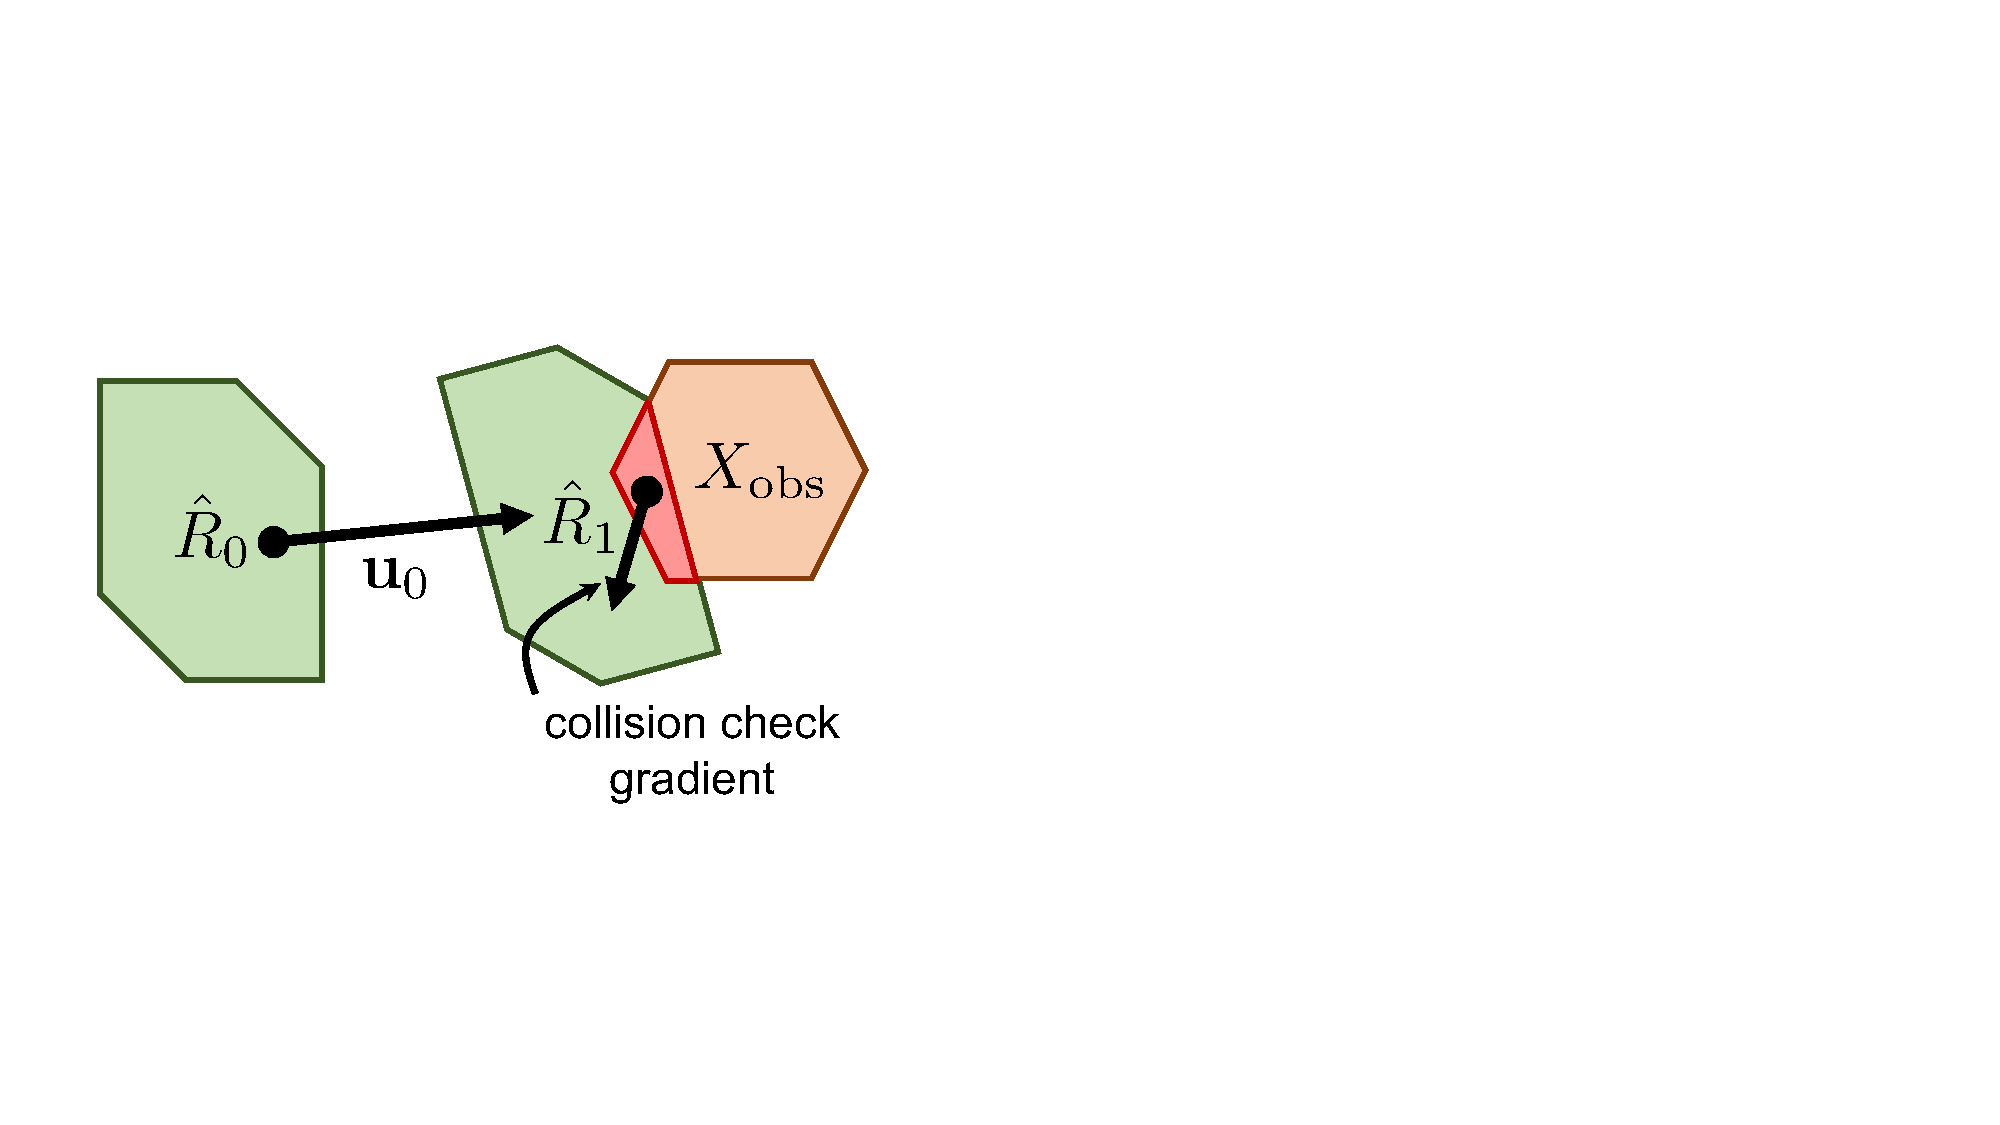
\includegraphics[scale=0.26]{Figures/collision_check_a.pdf}
%  \caption{}
%   \label{fig:Ng1} 
%\end{subfigure}
%\begin{subfigure}{0.49\columnwidth}
%\centering
%   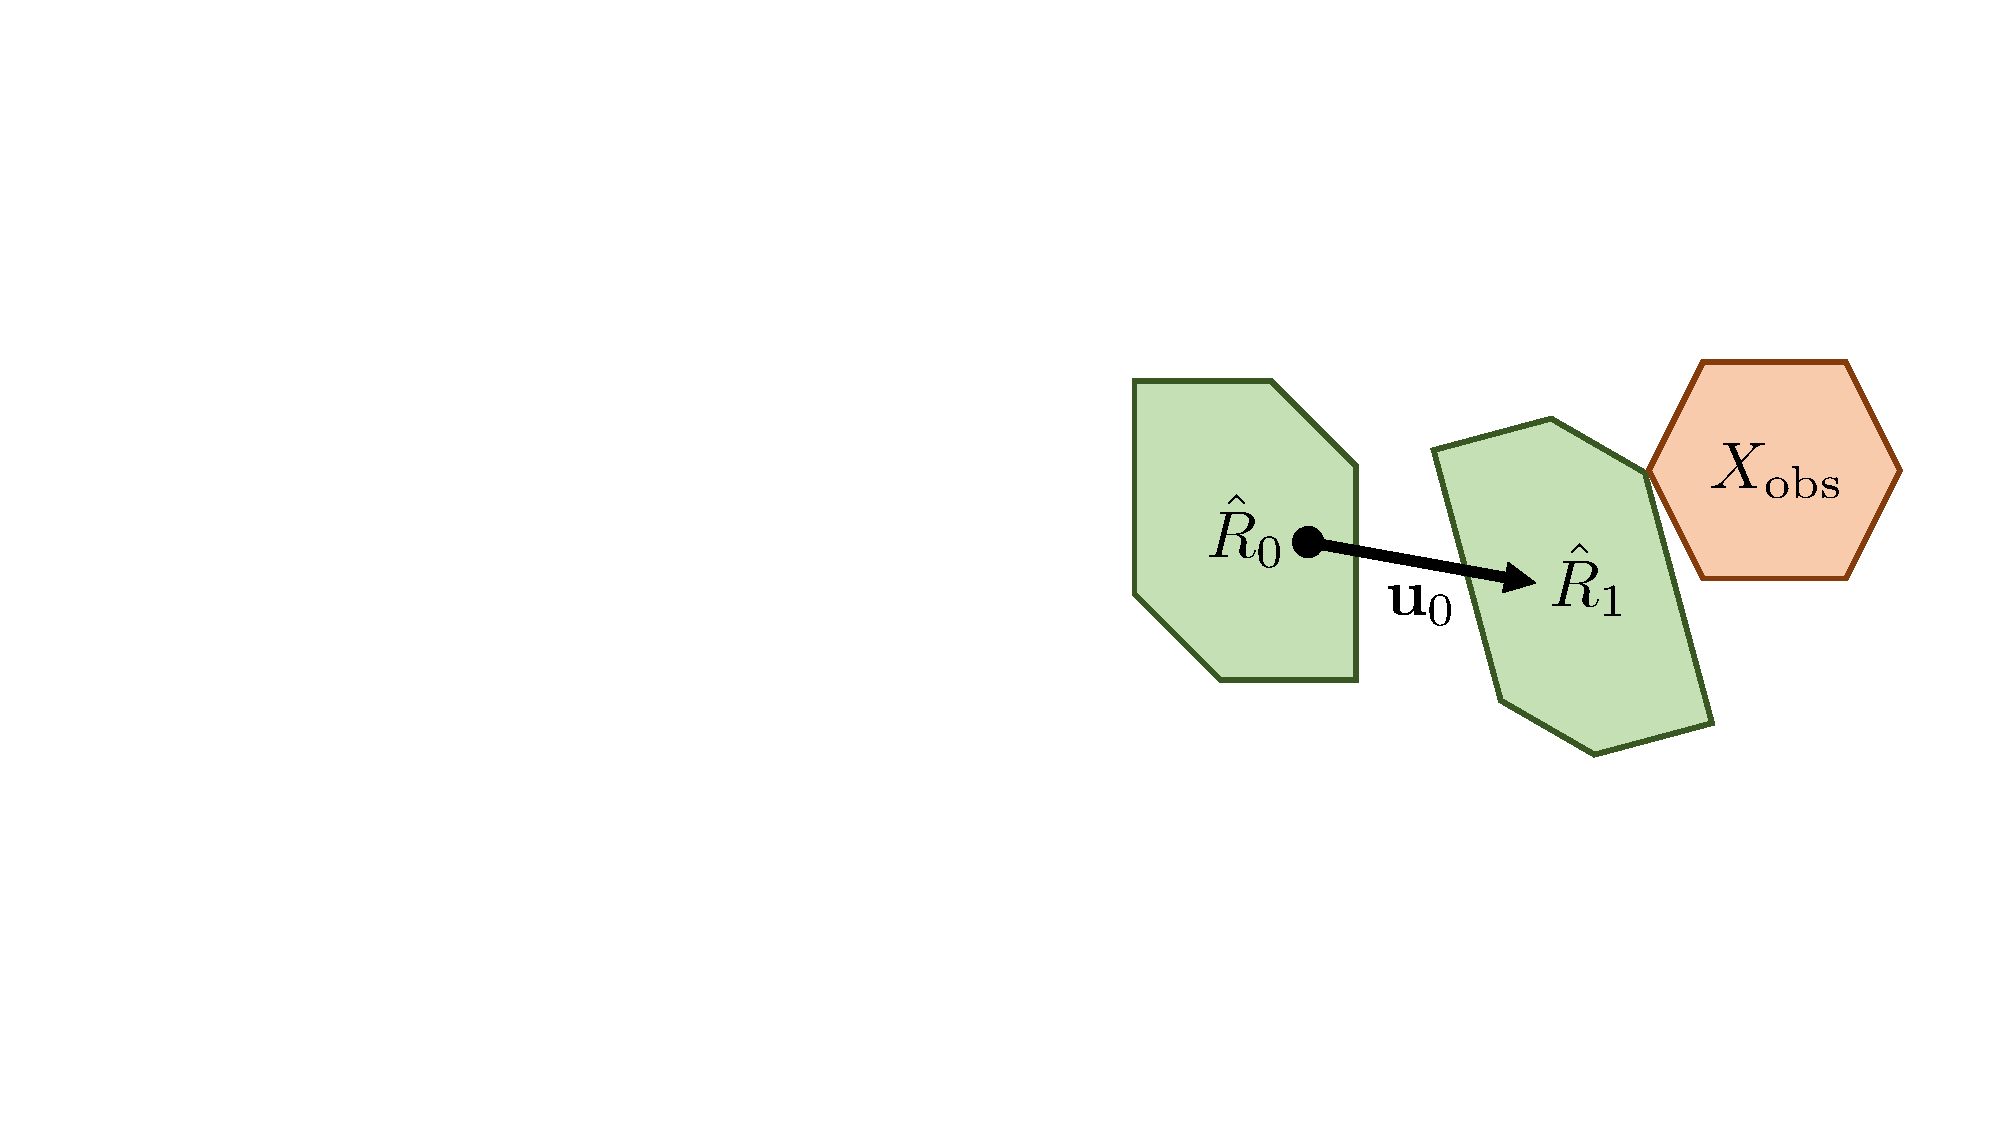
\includegraphics[scale=0.26]{Figures/collision_check_b.pdf}
%   \caption{}
%   \label{fig:Ng2}
%\end{subfigure}
%\caption{Our approach for pushing reachable sets, represented as zonotopes, out of intersection (see Alg. \ref{alg:adjust}).
%In (a), we compute the gradient of the collision check between the reachable set $\reachapprox_1$ and the obstacle $\statespace\obs$; in (b), we use constrained gradient descent to adjust $\action_0$ such that $\reachapprox_1\cap\statespace\obs = \emptyset$.}
%\label{fig:zonotope_intersection}
%\vspace{-2mm}
%\end{figure}

\begin{figure}
\centering     %%% not \center
\subfigure[]{\label{fig:Ng1}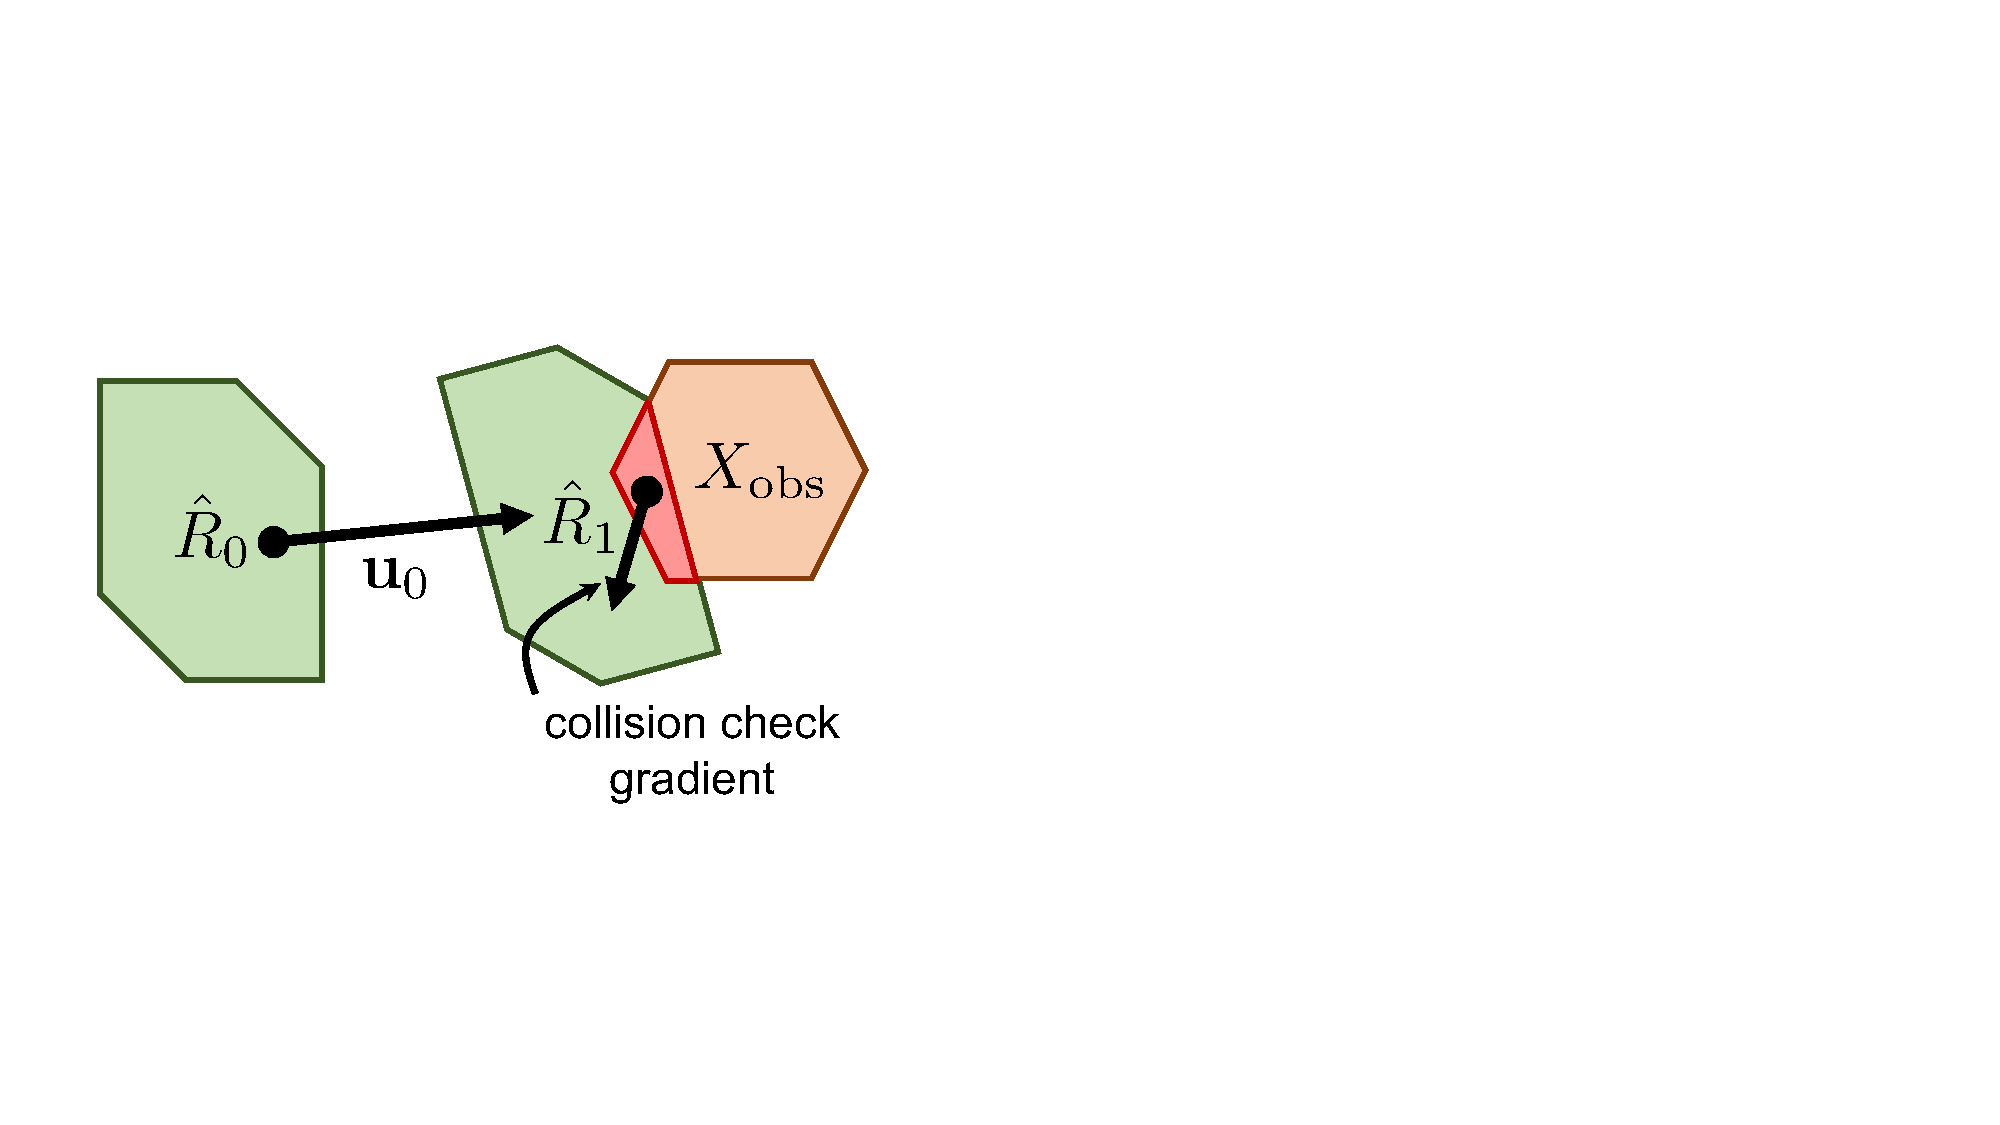
\includegraphics[width=0.4\columnwidth]{Figures/collision_check_a.pdf}}
\hspace{5mm}
\subfigure[]{\label{fig:Ng2}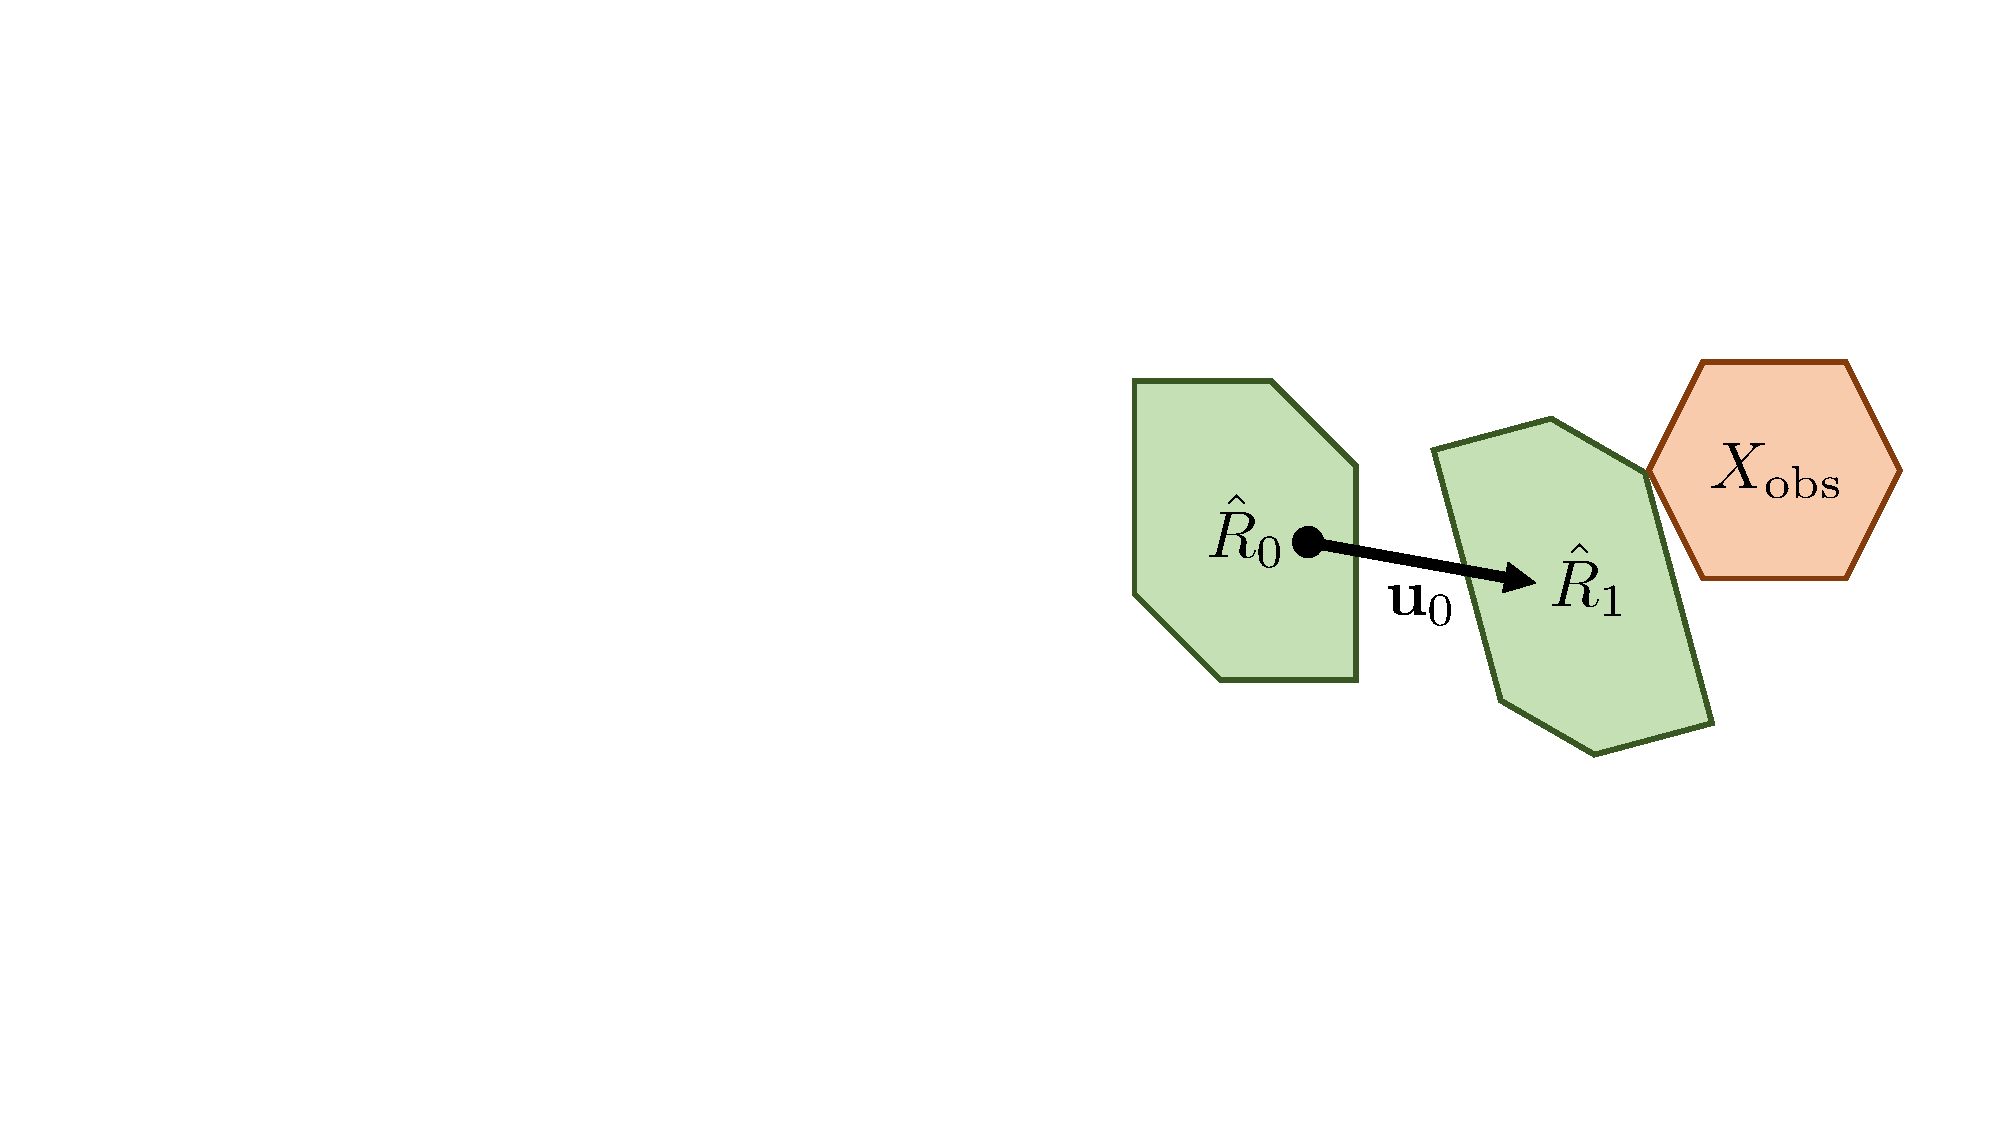
\includegraphics[width=0.4\columnwidth]{Figures/collision_check_b.pdf}}
\caption{We move zonotope reachable sets out of intersection (see Alg. \ref{alg:adjust}) by using the gradient of a collision check, shown in (a), to adjust $\action_0$ so the reachable sets are out of collision as shown in (b).} %between the reachable set $\reachapprox_1$ and the obstacle $\statespace\obs$; in (b), we use constrained gradient descent to adjust $\action_0$ such that $\reachapprox_1\cap\statespace\obs = \emptyset$.}
\label{fig:zonotope_intersection}
\vspace{-3mm}
\end{figure}


% \textbf{Differentiating the Collision Check.}~
We use gradient descent to move our reachable sets $\reachapprox_k$ out of collision.
Since we use \eqref{prog:collision_check} for collision checking, we differentiate its solution with respect to the problem parameters using \cite{amos2017optnet,chung2021constrained}.
Let $\hat{\ctr}_k$ denote the center of $\reachapprox_k$.
Per Algorithm \ref{alg:LipReachability}, $\reachapprox_k$ is a function of $\action_0,\cdots,\action_{k-1}$.
Let $(\coef\opt,v\opt)$ be an optimal solution to \eqref{prog:collision_check} when the problem parameters \tbold{(i.e., the input constrained zonotopes)} are $\reachapprox_k$ and an unsafe set.
Collision avoidance requires $v\opt > 1$ \cite[Prop. 2]{conf:const_zono}.
We compute the gradient $\nabla_{\RLaction_k} v\opt$ with respect to the input action (assuming a constant linearization point) using a chain rule recursion with $i = 0,\cdots,\nplan$ given by
\begin{align}\label{eq:collision_chain_rule}
    \nabla_{\RLaction_{h}} v\opt = \nabla_{\hat{\ctr}_k} v\opt
        \nabla_{\hat{\ctr}_{k - 1}} \hat{\ctr}_k
        \left(\prod_{j=h + 2}^{j = k - 1} \nabla_{\hat{\ctr}_{j - 1}} \hat{\ctr}_j\right) 
         \nabla_{\RLaction_{h}}  \hat{\ctr}_{h + 1},
\end{align}
with $h = k - i$.
The gradients of $\hat{\ctr}_k$ are given by
\begin{subequations}
\begin{align}
    &\nabla_{\hat{\ctr}_{k - 1}} \hat{\ctr}_k = (\vc{M}_{k - 1})_{(1:1+n),(1:1+n)},\ \regtext{and}
    \label{eq:collision_chain_rule_for_input_zono1} \\
    &\nabla_{u_{k - 1}} \hat{\ctr}_k = (\vc{M}_{k-1})_{:,(n+1:n+1+m)},
    \label{eq:collision_chain_rule_for_input_zono2}
\end{align}
\end{subequations}
where $\vc{M}_{k-1}$ is computed as in Algorithm \ref{alg:LipReachability}, Line \ref{ln:alglipMtilde}, and $n$ and $m$ are the state and action dimensions. 
After using  $\nabla_{\action_k}v\opt$ for gradient descent on $\action_k$, we project $\action_k$ to the set of feasible controls: $\proj_{\actionspace_k}(\action_k) = \argmin_{\vc{v} \in \actionspace_k} \left\{\norm{\action_k - \vc{v}}_2^2\right\}$.
The resulting controls may be unsafe, so we collision-check the final reachable sets at the end of Algorithm \ref{alg:adjust}.
% Using $\nabla_{\action_k}v\opt$ for gradient descent on $\action_k$ can cause ${\action_k \not\in U_k}$.
% Therefore, after each gradient step (Algorithm \ref{alg:adjust}, Line \ref{ln:adjust:get_gradient_and_step}), we project $\action_k$ into $\actionspace_k$ using a quadratic program: $\proj_{\actionspace_k}(\action_k) = \argmin_{\vc{v} \in \actionspace_k} \left\{\norm{\action_k - \vc{v}}_2^2\right\}$.
% Finding $\nabla_{\action_k}v\opt$ requires constrained gradient descent because we have constraints on the input actions.
% The problem in \eqref{eq:collision_chain_rule} can be solved either using projection or proximal operators since it is a convex optimization problem.

\begin{algorithm}[t]
\caption{Adjusting Unsafe Actions}
\label{alg:adjust}

\KwInput{plan $\plan_k = (\action_j)_{j=k}^{\nplan}$, obstacles $\statespace\obs$, initial reachable set $\reachapprox_k$, step size $\gamma$, time limit $t\lbl{max}$, time steps required to stop $n\brk$} 
// note $\plan_k$ has failsafe $\action\brk$ for all $j > k+\nplan$

$\plan\safe \leftarrow \plan_k$ // initialize with given plan

\For{$j = k:(k+\nplan + n\brk)$\label{ln:adjust:for_loop}}{
    \While{time limit not exceeded\label{ln:adjust:while_loop}}{
        $(\reachapprox_j)_{j=k}^{k+\nplan} \leftarrow \reachfunc{\reachapprox_j,\plan\safe}$ // use Alg. \ref{alg:LipReachability} \label{ln:adjust:reach}
    
        $v\opt \leftarrow $ collision check $\reachapprox_j \cap \statespace\obs$ using \eqref{prog:collision_check} \label{ln:adjust:collision_check}
        
        \uIf{$v\opt \leq 1$ (i.e., in collision)}{        
            $\action_j \leftarrow \proj_{\actionspace_j}\left(\action_j + \gamma \nabla_{\action_j} v\opt\right)$ // using \eqref{eq:collision_chain_rule} \label{ln:adjust:get_gradient_and_step}
            
            %$\action_j \leftarrow \proj_{\actionspace_j}(\action_j)$ \label{ln:adjust:project}
            
            %$\plan\safe\idx{j} \leftarrow \action_j$ // update current action \label{ln:adjust:update_action}
        }
        % \uElseIf{$\vcstate_n$ is not stopped}{
        %     $\action_j \leftarrow \tfrac{n-j}{n}\action_j + \tfrac{j}{n}\action\brk$ // add failsafe \label{ln:adjust:add_failsafe}
        % }
        \Else{
            \textbf{break} and restart inner while loop \label{ln:adjust:break_while_loop}
        }
    }
}

\eIf{all $\reachapprox_j \cap \statespace\obs = \emptyset$ and $\vcstate_n$ is stopped\label{ln:adjust:check_if_safe}}{
    % $p \leftarrow \sum_{k=0}^n \norm{\plan\idx{k} - \plan\safe\idx{k}}_2$ // compute penalty
    
    \textbf{return} $\plan\safe = (\action_j)_{j=k}^{\nplan}$ // found new safe plan% and $p$
}{
    \textbf{return} error ``unsafe'' // failed to find safe plan\label{ln:adjust:return_unsafe}
}
\end{algorithm}



\begin{figure*}[t]
\centering     %%% not \center
\begin{subfigure}[h][\tbold{Turtlebot3 Environment}]{\label{fig:tb_env}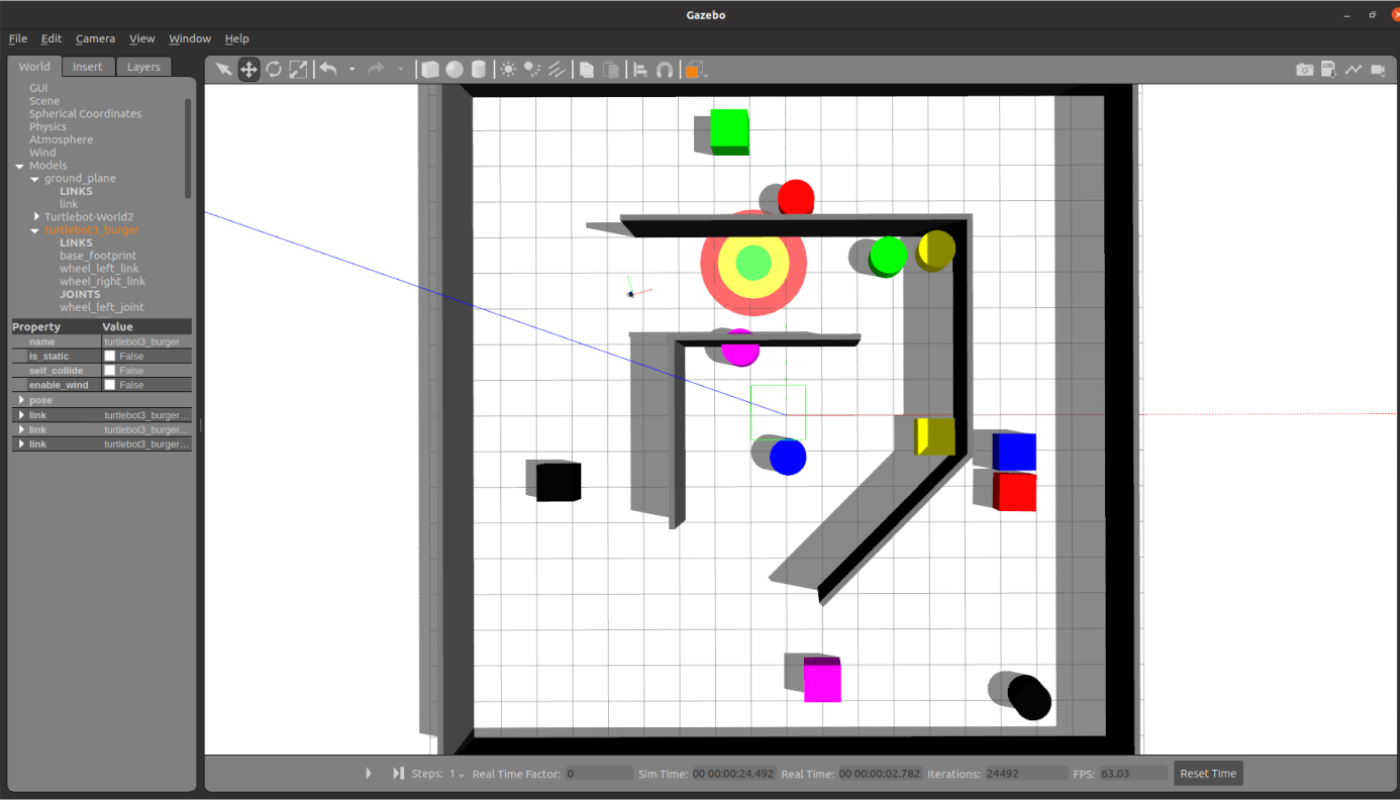
\includegraphics[scale=0.1]{Figures/Turtlebot-Env.png}}
\end{subfigure}
\begin{subfigure}[h][\tbold{Quadrotor Environment}]{\label{fig:quad_env}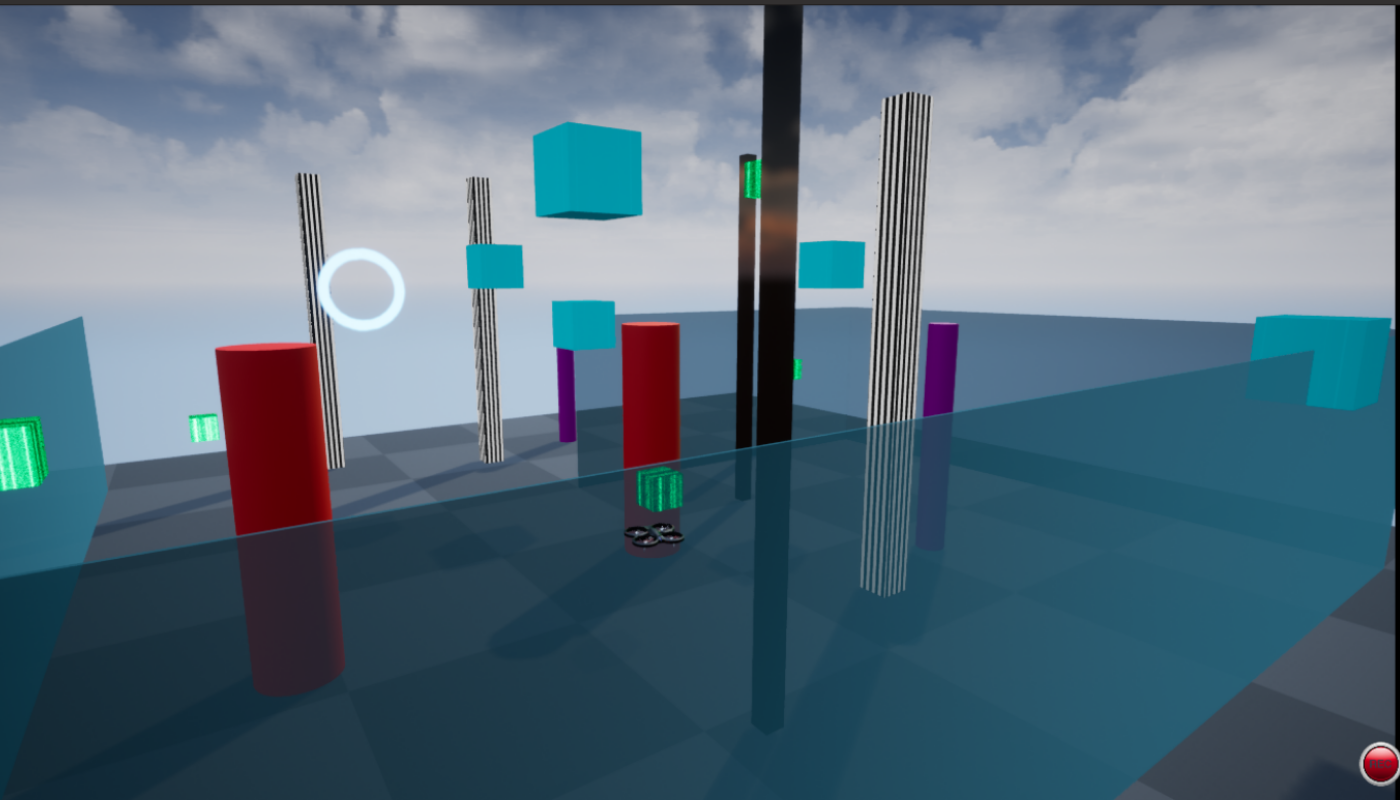
\includegraphics[scale=0.1]{Figures/Quadrotor-Env.png}}
\end{subfigure}
\begin{subfigure}[h][\tbold{Hexarotor Environment}]{\label{fig:hex_env}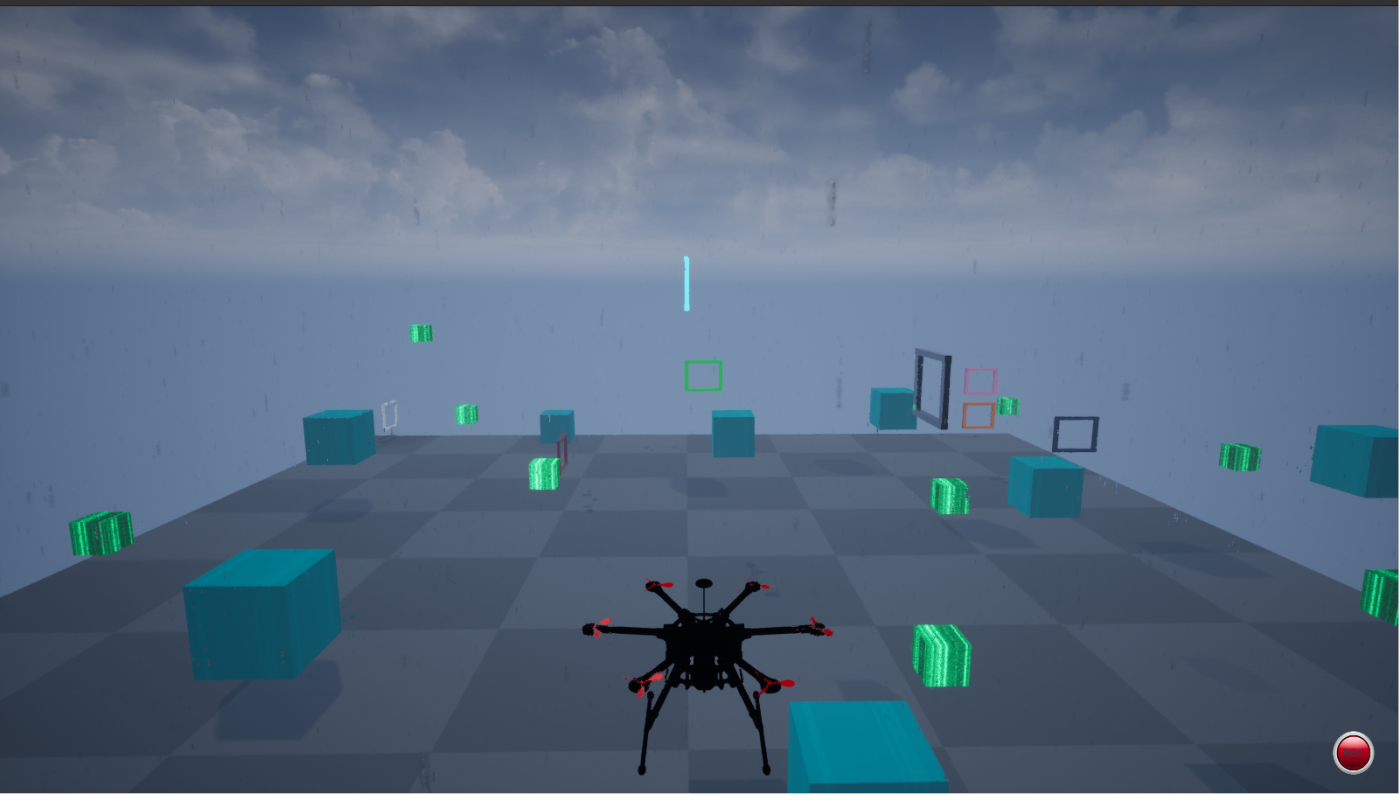
\includegraphics[scale=0.1]{Figures/Hexarotor-Env.png}}
\end{subfigure}
%\hspace{10mm}
%\subfigure[Arrival and collisions rates are in bold and dashed lines, respectively.]{\label{fig:Ng2}\includegraphics[scale=0.25]{Figures/turtlebot_safety.png}}
\caption{\tbold{Evaluation Environments.}}
\label{fig:sim_envs}
\vspace{-5mm}
\end{figure*}

 \subsection{Analyzing Safety}
%\textbf{Analyzing Safety.}
We conclude this section by formalizing the notion that BRSL enables safe RL.

\begin{theorem}\label{thm:BRSL_is_safe}
Suppose the assumptions on the robot and environment from Section \ref{sec:pb} all hold, and, at time $k = 0$, the robot is \tbold{at safe state}.
Suppose also that, at each time $k > 0$, the robot \tbold{rolls out} a new $\plan_k$, then adjusts the plan using Algorithm \ref{alg:adjust}.
Then, the robot is guaranteed to be safe at all times $k \geq 0$.
\end{theorem}
\begin{proof}
We prove the claim by induction on $k$.
At time $0$, the robot can apply $\action\brk$ to stay safe for all time.
Assume a safe plan exists at time $k \in \N$.
Then, if the output of Algorithm \ref{alg:adjust} is unsafe (no new plan found), the robot can continue its previous safe plan; otherwise, if a new plan is found, the plan is safe for three reasons.
First, the black-box reachability in Algorithm \ref{alg:LipReachability} is guaranteed to contain the true reachable set of the system \cite[Theorem 2]{alanwar2020data_conf}, because process noise is bounded by a zonotope as in Assumption \ref{assumption:noise_zonotope}.
Second, when adjusting an unsafe plan with Algorithm \ref{alg:adjust}, the zonotope collision check is guaranteed to always detect collisions \cite[Prop. 2]{conf:const_zono} to assess if $\reachapprox_j \cap \statespace\obs$ is empty for each time step $j$ of the plan.
Third, Algorithm \ref{alg:adjust} requires that, after $\nplan$ timesteps, the robot is stopped, so the new plan contains a failsafe manuever, and the robot can safely apply $\action\brk$ for all time $j \geq k+\nplan$.
\end{proof}



% \tbold{We note that the accuracy of the environment model, trained online, does not affect the above result.
% This is because we enforce safety via data-driven reachability; so, Theorem \ref{thm:BRSL_is_safe} will hold as long as the data (collected before runtime) are still representative of the robot's dynamics at runtime.
% We leave updating the data online for future work.}
We note that the accuracy of the environment model, trained online, does not affect safety; Theorem \ref{thm:BRSL_is_safe} holds as long as the offline data are representative of the robot's dynamics at runtime.
We leave updating the data online for future work.

% Next, we evaluate BRSL numerically.
\begin{figure*}
\centering     %%% not \center

\begin{subfigure}[h][Turtlebot3 Reward]{\label{fig:turtlebot_reward}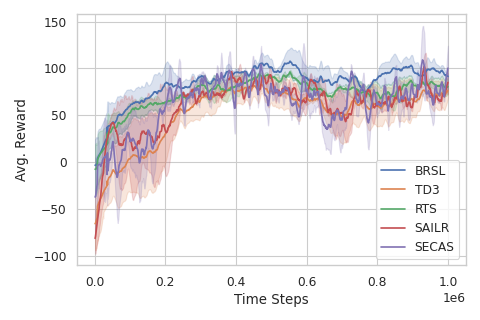
\includegraphics[scale=0.25]{Figures/Turtlebot3_reward.png}}
\end{subfigure}
\begin{subfigure}[h][Quadrotor Reward]{\label{fig:drone_reward}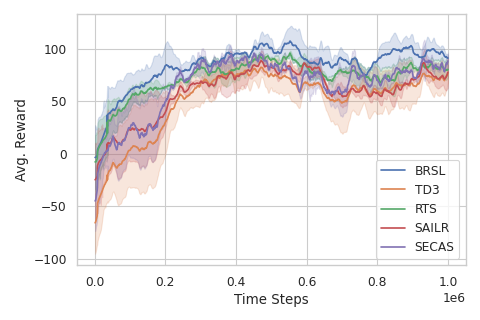
\includegraphics[scale=0.25]{Figures/Quadrotor_reward.png}}
\end{subfigure}
\begin{subfigure}[h][Point Reward]{\label{fig:point_reward}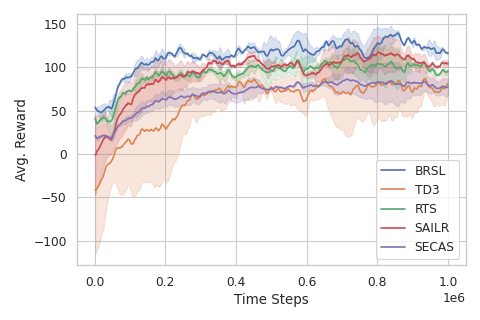
\includegraphics[scale=0.25]{Figures/Point_reward.png}}
\end{subfigure}
\begin{subfigure}[h][\tbold{Hexarotor Reward}]{\label{fig:hexarotor_reward}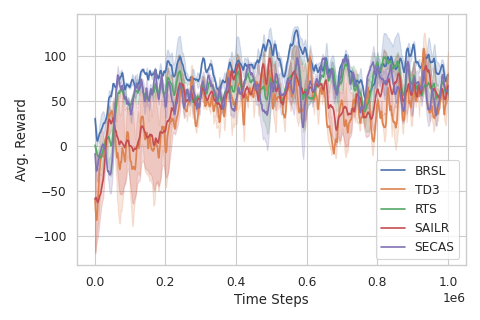
\includegraphics[scale=0.25]{Figures/Hexarotor_reward.png}}
\end{subfigure}
%\hspace{10mm}
%\subfigure[Arrival and collisions rates are in bold and dashed lines, respectively.]{\label{fig:Ng2}\includegraphics[scale=0.25]{Figures/turtlebot_safety.png}}

\caption{Average reward over time of BRSL, RTS \cite{conf:modelBasedReachRL}, SAILR \cite{wagener2021safe}, and a vanilla TD3 baseline for each of our experiments.}
\label{fig:sim_results}
\vspace{-2mm}
\end{figure*}

\begin{table*}[ht]
\caption{Goal-based experiment results (best values in bold)}
\label{tbl:comparison}
\vspace{-3mm}
\centering
\resizebox{1.98\columnwidth}{!}{\begin{tabular}{ c|c|c|c|c|c||c|c|c|c|c } 
 %\hline
 & \multicolumn{5}{c||}{Turtlebot} & \multicolumn{5}{c}{Quadrotor} \\
 & BRSL & RTS & SAILR & \tbold{SECAS}&Baseline  & BRSL & RTS & SAILR & \tbold{SECAS}& Baseline  \\
 \hline
 Goal Rate [\%] &
    \textbf{57} & 52 & 48 & \tbold{53} & 42  &
    \textbf{76} & 66 & 61 & \tbold{59} & 54 \\
 Collision Rate [\%] &
    \textbf{0.0} & \textbf{0.0} & 7.3 & \tbold{\textbf{0.0}} &48 
    &\textbf{0.0} & \textbf{0.0} & 9.2& \tbold{\textbf{0.0}} & 59\\
 Mean/Max Speed [m/s] & 
    .07 / \textbf{0.18} & 0.05 / 0.15 & .07 / 0.17 & \tbold{.06 / 0.15} &\textbf{.08} / \textbf{.18} & 
    3.6 / \textbf{7.9} &  3.3 / 7.8 & \textbf{3.7} / \textbf{7.9} & \tbold{3.2 / 7.8} & \textbf{3.7} / \textbf{7.9}\\
 Mean Reward &
    \textbf{86} & 78 & 68 & \tbold{66} & 63 &
    \textbf{82} & 73 & 61 & \tbold{68} & 57 \\
 Mean $\pm$ Std. Dev.  &
    \multirow{2}{*}{50.41 $\pm$ 20.5} & \multirow{2}{*}{100.74 $\pm$ 60.5} & \multirow{2}{*}{30.53 $\pm$ 10.8} & \tbold{\multirow{2}{*}{22.4 $\pm$ 14.66}} & \multirow{2}{*}{\textbf{10.21} $\pm$ 10.05} &
    \multirow{2}{*}{60.33 $\pm$ 20.34} & \multirow{2}{*}{260.85 $\pm$ 140.67} & \multirow{2}{*}{45.31 $\pm$ 20.84} & \tbold{\multirow{2}{*}{39.7 $\pm$ 34.08}} & \multirow{2}{*}{\textbf{20.63} $\pm$ 30.2} \\
    Compute Time [ms] &&&&&&& &&\\
 \hline
    \end{tabular}}
\vspace{-2mm}
\end{table*}

\begin{table*}[ht]
    \caption{Path Following Results (best values in bold)}
    \label{tbl:point_robot}
    \vspace{-2mm}
    \centering
    \resizebox{1.98\columnwidth}{!}{\begin{tabular}{ c|c|c|c|c|c||c|c|c|c|c|c}
    & \multicolumn{5}{c||}{Point Environment} & \multicolumn{5}{c}{\tbold{Hexarotor}} \\
         & BRSL & RTS & SAILR &\tbold{SECAS} &Baseline & \tbold{BRSL} & \tbold{RTS} & \tbold{SAILR} &\tbold{SECAS} &\tbold{Baseline}\\
         \hline
         Collisions [\%] &
            \textbf{0.0} & \textbf{0.0} & 4.9 & \tbold{\textbf{0.0}} &11.4 & \tbold{\textbf{0.0}} & \tbold{2} & \tbold{14} & \tbold{7} & \tbold{63} \\
         Mean Speed [m/s] & 
            0.76 & 0.72 & 0.78 & \tbold{0.68} &\textbf{0.86} & \tbold{3.81} & \tbold{3.4} & \tbold{3.84} & \tbold{3.1} & \tbold{\textbf{3.94}} \\
         Max Speed [m/s] & 
            \textbf{2.00} & 1.89 & \textbf{2.00} & \tbold{1.74} &\textbf{2.00} & \tbold{8.4} & \tbold{8.1} & \tbold{8.2} & \tbold{7.95} & \tbold{\textbf{8.7}} \\
         Mean Reward &
            \textbf{118} & 93 & 88 & \tbold{78} &73 & \tbold{\textbf{84}} & \tbold{78} & \tbold{69} & \tbold{62} & \tbold{57}\\
         Compute Time [ms] &
            30.0 $\pm$ 10.2 & 60.18 $\pm$ 20.09 & 20.49 $\pm$ 10.34 & \tbold{16.42 $\pm$ 8.7} &\textbf{8.64} $\pm$ 1.14 & \tbold{71.93 $\pm$ 34.52} & \tbold{290.96 $\pm$ 157.24} & \tbold{67.86 $\pm$ 22.34} & \tbold{48.53 $\pm$ 28.69} & \tbold{\textbf{32.79 $\pm$ 27.6}} \\
         \hline
    \end{tabular}}
\vspace{-2mm}
\end{table*}


\section{Evaluation} \label{sec:eval}

%\subsection{Safe Robot Navigation to a Goal}
We evaluate BRSL on two types of environments: safe navigation to a goal (a Turtlebot in Gazebo and a quadrotor platform in Unreal Engine $4$), and path following (a point mass based on \cite{achiam2017constrained,wagener2021safe} and a hexarotor in wind in Unreal Engine $4$).
Figure \ref{fig:sim_envs} shows example environments.
%To test the robustness of BRSL, we subject the hexarotor to uncertain wind, which violates Assumption \ref{assumption:stop}, to test the robustness of BRSL.
All code is run on a desktop computer with an Intel i5 11600 CPU and a RTX 3060 GPU. 
%\footnote{We plan to make the code open-source after publication.}.
Our code is available \href{https://github.com/Mahmoud-Selim/Safe-Reinforcement-Learning-for-Black-Box-Systems-Using-Reachability-Analysis}{\underline{\color{blue}{online}}}.
We aim to assess the following:
(a) How does BRSL compare against other safe RL methods (RTS \cite{conf:modelBasedReachRL}, SAILR \cite{wagener2021safe}, and SECAS \cite{dalal2018safe})?
(b) How conservative is BRSL?
(c) Can BRSL run in real time?
% \begin{itemize}
%     \item How does BRSL compare against a vanilla baseline (unsafe) RL agent and other safe RL methods (RTS \cite{conf:modelBasedReachRL}, SAILR \cite{wagener2021safe}, \tbold{and (SECAS) \cite{dalal2018safe}}) in terms of reward and safety?
%     \item How conservative is BRSL in environments where high reward states are near unsafe regions?
%     \item Can BRSL be implemented in real time for safety-critical systems?
% \end{itemize}

% \subsection{Setup}
\textbf{Setup.}
We use TD3 \cite{conf:TD3} as our RL agent, after determining empirically that it outperforms SAC \cite{conf:SAC} and DDPG \cite{conf:DDPG}. %(we justify this choice in the supplementary section).
We randomly initialize the policy.
Since the agent outputs continuous actions, to aid the exploration process, we inject zero-mean Gaussian noise with a variance of $0.5$ that is dampened each time step.
Note that this does not affect safety since our safety layer adjusts the output of the RL agent.

For each robot, to perform reachability analysis with Algorithm \ref{alg:LipReachability}, we collect $500$ time steps of noisy state/input data (as per \eqref{eq:data}) offline in an empty environment while applying random control inputs.
We found this quantity of data sufficient to ensure safety empirically; we leave a formal analysis of the minimum amount of data for future work.

We parameterize the environment \tbold{model} as an ensemble of neural networks, each modeling a Gaussian distribution over future states and observations.
Each network has $4$ layers, with hidden layers of size 200, and leaky ReLU activations with a negative slope of $0.01$.
We use a stochastic model wherein the ensemble predicts the parameters of a probability distribution, which is sampled to produce a state as in \cite{chua2018deep}.


% \subsubsection{Goal-Based Environments
\textit{Goal-Based Environments.}
The Turtlebot 3 and the quadrotor seek to navigate to a random circular goal region $\statespace\goal \subset \statespace$ while avoiding randomly-generated obstacles $\statespace\obs \subset \statespace$. %, as shown in Fig.~\ref{fig:turtleee} for the Turtlebot and Fig.~\ref{fig:droneee} for the quadrotor.
% Both Turtlebot's and the quadrotor's goals are randomly selected at the beginning of each episode.
Each robot starts in a safe location at the center of the map.
Each task is episodic, ending if the robot reaches the goal, crashes, or exceeds a time limit.
Both robots have uncertain, noisy dynamics as in \eqref{eq:sys}.
We discretize time at $10$ Hz.

The Turtlebot's control inputs are longitudinal velocity in $[0.00,0.25]$ m/s and angular velocity in $[-0.5, 0.5]$ rad/s (these are the bounds of $\actionspace_k$).
The robot has wheel encoders, plus a planar lidar that generates $18$ range measurements evenly spaced in a $180^\circ$ arc in front of the robot.
The robot requires $\nbrk = 6$ time steps to stop, so we set $\nplan = 8$.

The quadrotor control inputs are commanded velocities up to 5 m/s in each spatial direction at each time step.
\tb{We note that we also experimented with learning low-level rotor speeds versus high-level velocity commands, and found that the velocity commands created the fairest testing conditions across all agents}. The robot is equipped with an IMU and a 16-channel lidar which receives range measurements around the robot in a $50^\circ$ vertical arc and a $360^\circ$ horizontal arc.
The robot has $\nbrk = 10$, so we set $\nplan = 11$.

%We use the following reward for goal-based environments:
%\newcommand{\indic}{\mathbb{I}}
%\begin{align}\begin{split}
%    \rewfunc(\RLstate_k,\RLaction_k) =
%    &+10^3\cdot \indic\left(\vcstate_k \in X\goal\right) +\\
%    &-20\cdot d\left(\vcstate_k,\statespace\goal\right)+ \\
%    &-10^3\cdot\indic\left(\RLaction_k\ \text{is unsafe}\right), %\end{split}
%\end{align} 
%where $\indic(\cdot)$ returns 1 if its argument is true or 0 otherwise, $d(\cdot,X\goal)$ returns the Euclidean distance to the center of the goal region, and the safety of $\RLaction_k$ is checked using the reachable set of the RL agent's plan (before adjustment).
%The robot position is estimated from the odometry of the robot.


%\TODO{These robot-specific details should be moved to the supplement.}



% \subsection{Choosing an RL Agent}
%\TODO{This subsection can be moved to the supplement; in this section, we just need to say we're using TD3.}
%We chose TD3 \cite{conf:TD3} as our RL agent. %(we justify this choice in the supplementary section).
%Since the agent outputs continuous actions, to aid the exploration process, we inject zero-mean Gaussian noise with a variance of $0.5$ that is dampened by a factor of $0.99995$ per time step.




% \begin{figure*}[ht]
% \vspace{-0.05cm}
%     \centering
%     % \begin{tabular}{ p{0.330\textwidth}  p{0.330\textwidth} p{0.330\textwidth}}
%     % \resizebox{0.32\textwidth}{!}{
%             \begin{subfigure}[h]{0.33\textwidth}
%      \centering
%         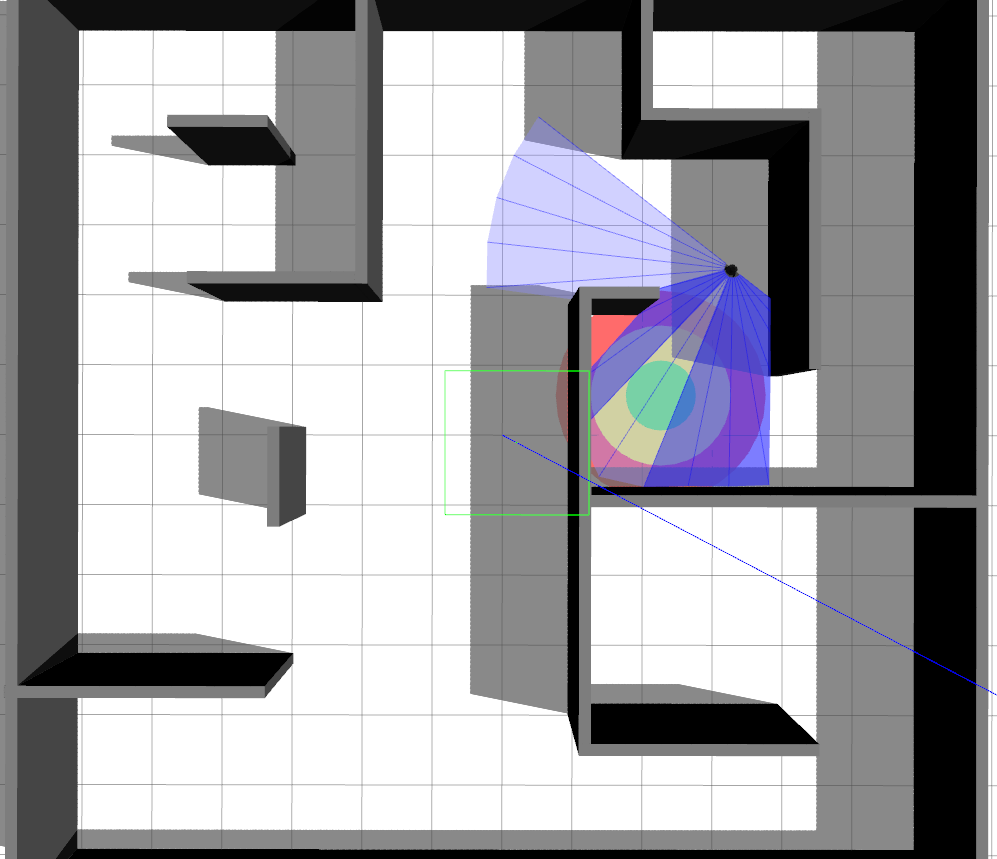
\includegraphics[scale=0.11]{Figures/turtleee.png}
%         \caption{Turtlebot Environment. The goal for the robot (black dot) is to reach the green circle.}%It is designed so that unsafe RL experience many collisions.} %%The goal is the green circle. Its position is also changed at each episode}
%         \label{fig:turtleee}
%     \end{subfigure}
%     %   } 
% %   &
% %   \resizebox{0.32\textwidth}{!}{
%             \begin{subfigure}[h]{0.33\textwidth}
%      \centering
%         \includegraphics[scale=0.33]{Figures/turtlebot_reward.png}
%         \caption{Turtlebot reward comparisons.}% Both safe agents learn to achieve higher reward than the unsafe TD3}
%         \label{fig:safe_agent}
%     \end{subfigure}
%     %  }
%     %     &
% %   \resizebox{0.32\textwidth}{!}{
%             \begin{subfigure}[h]{0.33\textwidth}
%      \centering
%         \includegraphics[scale=0.32]{Figures/turtlebot_safety.png}
%         \caption{Arrival and collisions rates are in bold and dashed lines, respectively.} %Both BRSL and RTS have no collisions and baseline TD3 learns to avoid obstacles. All three agents learn to arrive at goals with time.
%         \label{fig:img_with_vars}
%     \end{subfigure}
% %      }
% %  \end{tabular}
% \caption{Comparison between TD3, BRSL, and RTS in the Turtlebot navigation.}
%     \label{fig:turtleee3fig}%\vspace{-4mm}
%     \vspace{-4mm}
% \end{figure*}

% \subsubsection{Path Following Environments}
\textit{Path Following Environments.}
These experiments assess BRSL's conservativeness is by placing the highest reward adjacent to obstacles.

The goal for the point robot is to follow a circular path of radius $r$ as quickly as possible while constrained to a region smaller than the target circle.
The point robot is a 2-D double integrator with position and velocity as its state: $\vcstate_k = (x_k,y_k,\dot{x}_k,\dot{y}_k)$.
It has a maximum velocity of 2 m/s, and its control input is acceleration up to 1 m/s$^2$ in any direction.
We use these dynamics as in \cite{achiam2017constrained,wagener2021safe} to enable a fair test against other methods that require a robot model.
We define a box-shaped safe set (the complement of the obstacle set) as $\statespace\safe = \{\vcstate_k \in \statespace : |x_k| \le x_{\max},  |y_k| \le y_{\max}\}$, with $\norm{(x_{\max}, y_{\max})}_2 < r$.
We use a reward that encourages traveling quickly near the unsafe set: $\rewfunc (\RLstate_k,\RLaction_k) = \frac{(\dot{x}_k, \dot{y}_k) \cdot (-y_k, x_k)}{1 + \big| \norm{(x_k, y_k)}_2 - r\big|}$.
% \begin{align}\begin{split}
%     \rewfunc (\RLstate_k,\RLaction_k) = \frac{(\dot{x}_k, \dot{y}_k) \cdot (-y_k, x_k)}{1 + \big| \norm{(x_k, y_k)}_2 - r\big|}.
% \end{split}\end{align}

The hexarotor has the same setup as the quadrotor, but with the addition of wind as an external disturbance.
The goal of the hexarotor is to pass through $10$ checkpoints in a fixed order while subject to wind (constant speed and direction) and randomly-placed obstacles.
Note, offline data collection was performed under wind conditions.
% As for the robot's action, it's a vector containing the horizontal and vertical accelerations of the robot. That is $\RLaction \in \mathbbm{R}^2 = (a_x, a_y)$.
%\TODO{explain what the control inputs and observations are for the point robot}


%\begin{figure}[t]
%\centering     %%% not \center
%\subfigure[Turtlebot Environment.]{\label{fig:turtlebo_env}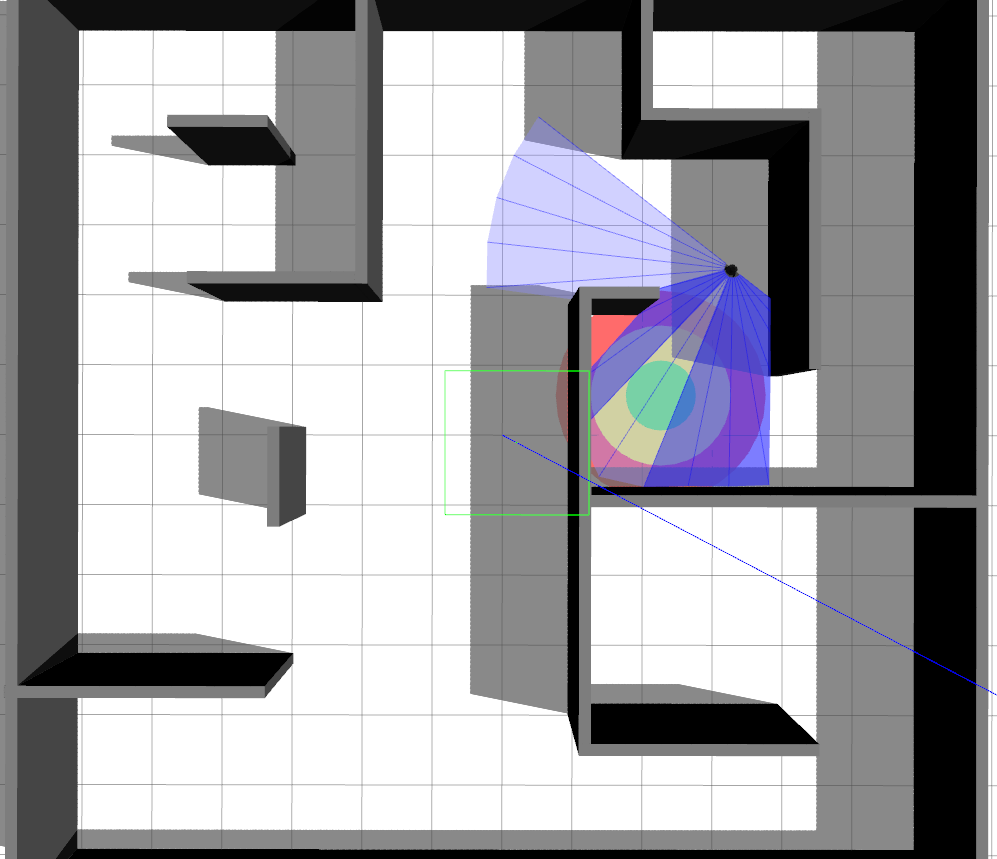
\includegraphics[scale=0.13]{Figures/turtleee.png}}
%\hspace{10mm}
%\subfigure[Turtlebot reward comparisons.]{\label{fig:turtlebot_reward}\includegraphics[scale=0.4]{Figures/turtlebot_reward.png}}
%\hspace{10mm}
%\subfigure[Arrival and collisions rates are in bold and dashed lines, respectively.]{\label{fig:Ng2}\includegraphics[scale=0.25]{Figures/turtlebot_safety.png}}
%\caption{Comparison between TD3, BRSL, and RTS in the Turtlebot navigation.}
%\label{fig:turtleee3fig}
%\end{figure}

% \begin{figure*}[!htbp]
% \vspace{-0.05cm}
%     \centering
%     % \begin{tabular}{ p{0.330\textwidth}  p{0.330\textwidth} p{0.330\textwidth}}
%     % \resizebox{0.32\textwidth}{!}{
%             \begin{subfigure}[h]{0.33\textwidth}
%      \centering
%         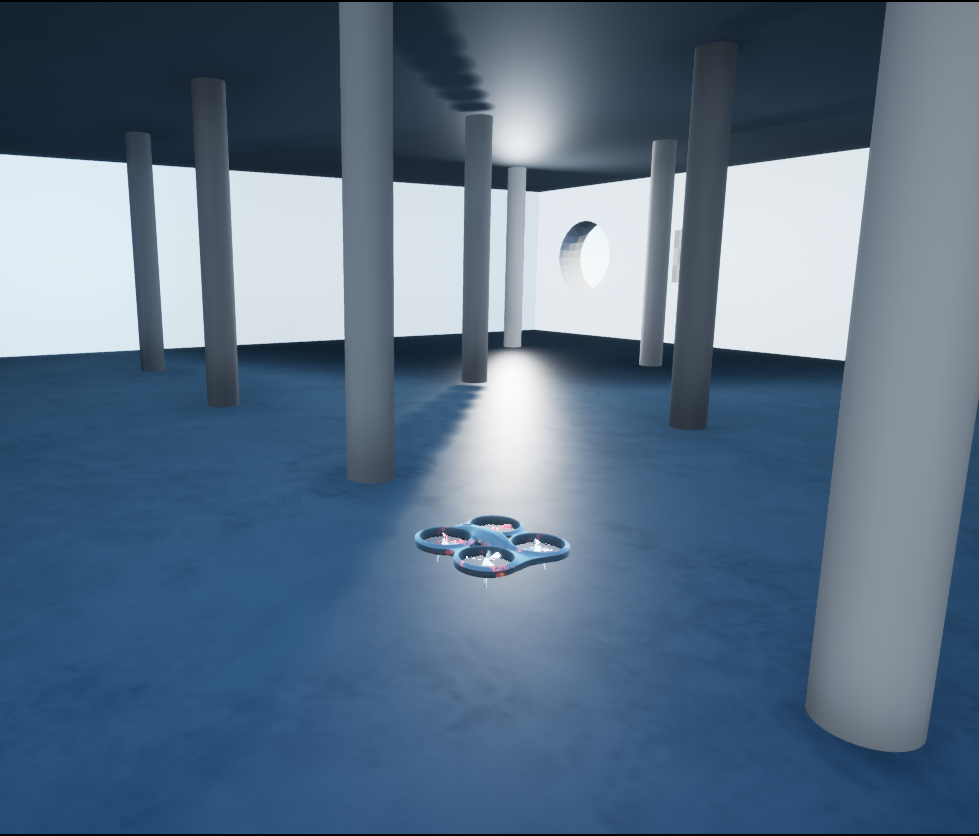
\includegraphics[scale=0.11]{Figures/droneee.png}
%         \caption{quadrotor Environment.
%         The goal is the circular hole in the wall.}
%         \label{fig:droneee}
%     \end{subfigure}
% %       } 
% %   &
% %   \resizebox{0.32\textwidth}{!}{
%             \begin{subfigure}[h]{0.33\textwidth}
%      \centering
%         \includegraphics[scale=0.33]{Figures/drone_reward.png}
%         \caption{quadrotor reward comparisons.}% Both safe agents learn to achieve higher reward than the unsafe TD3}
%         \label{fig:drone_reward}
%     \end{subfigure}
%     %  }
%     %     &
% %   \resizebox{0.32\textwidth}{!}{
%             \begin{subfigure}[h]{0.33\textwidth}
%      \centering
%         \includegraphics[scale=0.32]{Figures/drone_safety.png}
%         \caption{Arrival and collisions rates are in bold and dashed lines, respectively.}%. Both BRSL and RTS have no collisions and baseline TD3 learns to avoid obstacles. All three agents learn to arrive at goals with time.}
%         \label{fig:drone_safety}
%     \end{subfigure}
% %      }
% %  \end{tabular}
% \caption{Comparison between TD3, BRSL, and RTS in the quadrotor experiment.}
%     \label{fig:droneee3fig}%\vspace{-4mm}
%     \label{fig:drone_fig}
%     \vspace{-4mm}
% \end{figure*}

%\begin{figure}
%\centering     %%% not \center
%\subfigure[quadrotor Environment.]{\label{fig:drone_env}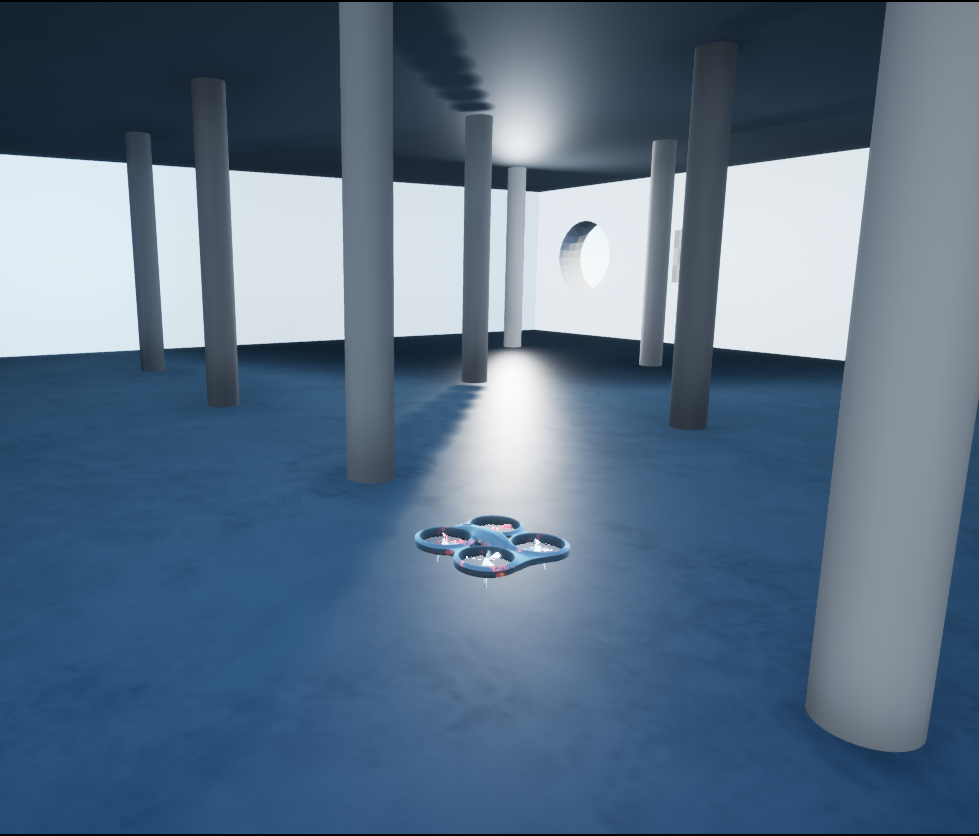
\includegraphics[scale=0.135]{Figures/droneee.png}}
%\hspace{10mm}
%\subfigure[quadrotor reward comparisons.]{\label{fig:drone_reward}\includegraphics[sca%le=0.4]{Figures/drone_reward.png}}
%\hspace{10mm}
%\subfigure[Arrival and collisions rates are in bold and dashed lines, respectively.]{\label{fig:Ng2}\includegraphics[scale=0.25]{Figures/turtlebot_safety.png}}
%\caption{Comparison between TD3, BRSL, and RTS in the %quadrotor experiment.}
%\label{fig:drone_fig}
%\end{figure}



% \subsection{Results and Discussion}
\textbf{Results and Discussion.}
\tb{The results are summarized in Tables \ref{tbl:comparison} and \ref{tbl:point_robot}, and in Figure \ref{fig:sim_results}.
%RTS is almost the same in terms of reward and arrival rate as our BRSL framework.
BRSL outperforms the other methods in terms of reward and safety, is not overly conservative, and can operate in real time, despite lacking a model of the robot \emph{a priori}.
While SAILR and the baseline RL agent achieved higher speeds, both experienced collisions, unlike BRSL, RTS, and SECAS.
In contrast to RTS, which chooses from a low-dimensional parameterized plans, BRSL outputs a more flexible sequence of actions.
Furthermore RTS' planning time increases with state space dimension due to computing a halfspace representation of reachable set zonotopes, which grows exponentially in the number of generators \cite{althoffphdthesis}.
BRSL avoids this computation by using \eqref{prog:collision_check}.
Instead, the quantity of data for BRSL determines the computation time of $\vc{M}_j$ from Algorithm \ref{alg:LipReachability}, used for reachability and adjusting unsafe actions.
Therefore, one can ensure the amount of data allows real time operation; choosing the data optimally is left to future work.
Finally, BRSL uses zonotopes to exactly represent safety constraints, whereas SECAS uses a more conservative first-order approximation.
This results in BRSL achieving higher reward with slightly slower computation time (but still fast enough for real time operation).}
% It is possible RTS can be more efficient with hyperparameter tuning; our focus is BRSL's real-time capability.

% \tb{
% We explain BRSL's performance advantages as follows.
% First, BRSL outputs a more flexible sequence of actions than RTS, which chooses from a low-dimensional parameterized set of plans.
% % Second, SAILR does not enforce hard safety constraints, unlike BRSL.
% Second, BRSL exactly represents safety constraints, whereas SECAS uses a more conservative first-order approximation.
% }
% \begin{table}[ht]
%     \caption{Mean $\pm$ std. dev. of computation time in seconds.}
%     \label{tab:runtimes}
%     \centering
%     \begin{tabular}{c | c | c | c | c }
%          Robot& BRSL & RTS & SAILR & Baseline \\
%          \hline
%          Turtlebot3 & 0.05 $\pm$ 0.02 & 0.10 $\pm$ 0.06 & 0.03 $\pm$ 0.01 & 0.01 $\pm$ 0.01 \\
%          Quadrotor & 6 $\pm$ 2 & 26 $\pm$ 14 & 4.5 $\pm$ 2 & 2 $\pm$ .3 \\
%          %Hexarotor (12/6) & x $\pm$ y & x $\pm$ y & x $\pm$ y & x $\pm$ y \\
%          Point & 3 $\pm$ 1 & 6 $\pm$ 2 & 2 $\pm$ 1 & .8 $\pm$ .07 \\
%          \hline
%     \end{tabular}
% \end{table}


\section{Conclusion}\label{sec:con}

This paper proposes the Black-box Reachability Safety Layer, or BRSL, for safe RL without having a system model \textit{a priori}.
BRSL ensures safety via data-driven reachability analysis and a novel technique to push reachable sets out of collision.
To enable the RL agent to make dynamics-informed decisions, BRSL also learns an environment model online, which does not affect the safety guarantee.
The framework was evaluated on four robot motion planning problems, wherein BRSL respects safety constraints while achieving a high reward over time in comparison to state-of-the-art methods.
For future work, we will explore continuous-time settings, reducing the conservativeness of our reachability analysis, and minimizing the amount of data needed to guarantee safety.

\bibliographystyle{IEEEtran}
\bibliography{ref} 
%\bibliographystyle{ACM-Reference-Format}
% \bibliography{ref}
% \bibliographystyle{icml2021}
% \clearpage

% \appendix
% \section{Implementation Details}

\subsection{Data Collection and Processing}
\subsubsection{Data Collection}
The data was collected by letting the agent choose random actions in an empty environment in both cases for $500$ time steps. Then, this data was saved and used again while running the agents in both the training and testing environments.

\subsubsection{Data Processing and Warping}~
BRSL heavily depends on data-driven reachability analysis.
Getting the most suitable data that covers the whole space has a crucial effect on how conservative BRSL's forward reachability analysis is.
This conservatism worsens when we calculate the forward reachable sets for many timesteps; that is, each time step makes the reachable set zonotopes much larger.

To mitigate this problem, we apply a small trick to reduce the reachability zonotopes' volume.
First, we note that the state-space can be warped in the collected data such that an upper and a lower limit is imposed without loss of generality (WLOG).
We can enforce the position of a robot, for example, to be confined only within $[0, 1]$ WLOG.
In our examples, the robot's dynamics are position-invariant.
This means that we can confine the offline collected data to be within this range. 
We find empirically that this strategy significantly reduces BRSL's conservatism without impeding safety guarantees.
% For the Turtlebot example, 500 data points were more than enough to get our framework running. 

%\subsection{Environment Mimic}

%\subsubsection{Architecture}

%\subsubsection{Training}
%The loss function used for training is...



%\subsection{RTS Implementation}

%\subsubsection{Turtlebot}
%The Turtlebot's high-fidelity model is...

%We use the following planning model...


%\subsubsection{Quadrotor}
%The high-fidelity model is...

%The wind is modeled as...

%We use the following planning model...


\subsubsection{Approximating the Lipschitz Constant}

Determining a Lipschitz constant $L^\star$ and covering radius $\delta$ is, in general, difficult.
In this work, we apply the method from \cite[Remark 9]{alanwar2020data}.
Assume that the data $\statedata_-$ and $\actiondata$ (as in \eqref{eq:data}) are evenly distributed in $\statespace\times\actionspace$ (which are assumed to be compact).
Let $Z = (\statedata_-, \actiondata)$.
Then we approximate upper bounds for $L^\star$ and $\delta$ as
\begin{align}
    \hat{L}^\star &= \max_{\vc{z}_i, \vc{z}_j \in Z, j \neq i} \frac{\norm{\dyn(\vc{z}_i) - \dyn(\vc{z}_j)}_2}{\norm{\vc{z}_i - \vc{z}_j}_2},\ \regtext{and} \\
    \hat{\delta} &= \max_{\vc{z}_i \in Z} \min_{\vc{z}_j \in Z, j \neq i} \norm{\vc{z}_i - \vc{z}_j}_2,
\end{align}
where $\vc{z}_i \in Z$ is a minor abuse of notation to denote choosing $\vc{z}_i$ as a state/action pair from the data matrices in $Z$.



\subsection{Experiments}

\subsubsection{RL Agent Choice}
To select an RL agent for our experiments, we run a preliminary evaluation of three different agents for both robots: TD3 \cite{conf:TD3}, SAC \cite{conf:SAC}, and DDPG \cite{conf:DDPG}.
The agents are trained in randomized environments for $10^5$ time steps.
We choose TD3 for subsequent simulations as it outperforms SAC and DDPG in terms of maximum cumulative reward for both robots.


\subsubsection{Environment Mimic Sampling Details}
\TODO{explain how to do sampling from the stochastic model}



\subsubsection{Turtlebot Details}

The Turtlebot's control inputs are longitudinal and angular velocities.
Its maximum longitudinal velocity is $0.25$ m/s, and its angular velocity lies within $[-0.5, 0.5]$ rad/s.
The Turtlebot is equipped with wheel encoders and with a planar lidar that generates $18$ noisy distance measurements evenly spaced in a $180^\circ$ arc in front of the robot.
The Turtlebot requires a maximum of  $\nbrk = 3$ time steps to execute a failsafe braking maneuver, so we set $\nplan = 4$.


\subsubsection{Quadcopter Details}

The quadcopter control input at each time is a commanded velocity in each spatial direction.
The quadcopter's maximum speed is $5$ m/s (in any direction).
It is equipped with an IMU and a 16-channel lidar which generates noisy point cloud data in a $50^\circ$ vertical FOV and a $360^\circ$ horizontal FOV (a $360^\circ$-arc around the robot). 
The robot requires $\nbrk = 5$ time steps (i.e., 1 s at our discretization of 5 Hz) to come to a stop from its maximum speed, so we set $\nplan = 5$.


\end{document}
